%%%%%%%%%%%%%%%%%%%%%%%%%%%%%%%%%%%%%%%%%%%%%%%%%%%%%%%%%%%%%%%%%%%%%%%%%%%%
% AGUJournalTemplate.tex: this template file is for articles formatted with LaTeX
%
% This file includes commands and instructions
% given in the order necessary to produce a final output that will
% satisfy AGU requirements, including customized APA reference formatting.
%
% You may copy this file and give it your
% article name, and enter your text.
%
%
% Step 1: Set the \documentclass
%


%% To submit your paper:
\documentclass[draft]{agujournal2019}
\usepackage{url} %this package should fix any errors with URLs in refs.
\usepackage{lineno}
\usepackage{float}
\usepackage{amsmath,amssymb,amsfonts}
\usepackage[inline]{trackchanges} %for better track changes. finalnew option will compile document with changes incorporated.
\usepackage{soul}
\linenumbers
%%%%%%%
% As of 2018 we recommend use of the TrackChanges package to mark revisions.
% The trackchanges package adds five new LaTeX commands:
%
%  \note[editor]{The note}
%  \annote[editor]{Text to annotate}{The note}
%  \add[editor]{Text to add}
%  \remove[editor]{Text to remove}
%  \change[editor]{Text to remove}{Text to add}
%
% complete documentation is here: http://trackchanges.sourceforge.net/
%%%%%%%

%\draftfalse

%% Enter journal name below.
%% Choose from this list of Journals:
%
% JGR: Atmospheres
% JGR: Biogeosciences
% JGR: Earth Surface
% JGR: Oceans
% JGR: Planets
% JGR: Solid Earth
% JGR: Space Physics
% Global Biogeochemical Cycles
% Geophysical Research Letters
% Paleoceanography and Paleoclimatology
% Radio Science
% Reviews of Geophysics
% Tectonics
% Space Weather
% Water Resources Research
% Geochemistry, Geophysics, Geosystems
% Journal of Advances in Modeling Earth Systems (JAMES)
% Earth's Future
% Earth and Space Science
% Geohealth
%
% ie, \journalname{Water Resources Research}

\journalname{JGR: Solid Earth}


\begin{document}

%% ------------------------------------------------------------------------ %%
%  Title
%
% (A title should be specific, informative, and brief. Use
% abbreviations only if they are defined in the abstract. Titles that
% start with general keywords then specific terms are optimized in
% searches)
%
%% ------------------------------------------------------------------------ %%



\title{A spectral boundary-integral method for faults and fractures in a poroelastic solid: Simulations of a rate-and-state fault with dilatancy, compaction, and fluid injection}

%% ------------------------------------------------------------------------ %%
%
%  AUTHORS AND AFFILIATIONS
%
%% ------------------------------------------------------------------------ %%

% Authors are individuals who have significantly contributed to the
% research and preparation of the article. Group authors are allowed, if
% each author in the group is separately identified in an appendix.)

% List authors by first name or initial followed by last name and
% separated by commas. Use \affil{} to number affiliations, and
% \thanks{} for author notes.
% Additional author notes should be indicated with \thanks{} (for
% example, for current addresses).

% Example: \authors{A. B. Author\affil{1}\thanks{Current address, Antartica}, B. C. Author\affil{2,3}, and D. E.
% Author\affil{3,4}\thanks{Also funded by Monsanto.}}

\authors{El\'ias Rafn Heimisson\affil{1,2}, Shengduo Liu\affil{3}, Nadia Lapusta\affil{2,3}, John Rudnicki\affil{4}}



\affiliation{1}{Swiss Seismological Service, ETH Zurich, Zurich, Switzerland}
\affiliation{2}{Division of Geological and Planetary Sciences, California Institute of Technology, Pasadena, CA, USA}
\affiliation{3}{Division of Engineering and Applied Science, California Institute of Technology, Pasadena, California, USA}
\affiliation{4}{Department of Civil and Environmental Engineering and Department of Mechanical Engineering, Northwestern University, Evanston, IL, USA}
%% Corresponding Author:
% Corresponding author mailing address and e-mail address:

% (include name and email addresses of the corresponding author.  More
% than one corresponding author is allowed in this LaTeX file and for
% publication; but only one corresponding author is allowed in our
% editorial system.)

% Example: \correspondingauthor{First and Last Name}{email@address.edu}

\correspondingauthor{El\'ias Rafn Heimisson}{elias.heimisson@sed.ethz.ch}

%% Keypoints, final entry on title page.

%  List up to three key points (at least one is required)
%  Key Points summarize the main points and conclusions of the article
%  Each must be 100 characters or less with no special characters or punctuation and must be complete sentences

% Example:
% \begin{keypoints}
% \item	List up to three key points (at least one is required)
% \item	Key Points summarize the main points and conclusions of the article
% \item	Each must be 100 characters or less with no special characters or punctuation and must be complete sentences
% \end{keypoints}

\begin{keypoints}
\item We present a novel spectral boundary-integral method (SBIM) for a 2D poroelastic solid
\item We solve for fault slip with fully-coupled dilatancy and injection on a rate-and-state fault
\item The method is applied to study the influence of several parameters on fault stability
\end{keypoints}

%% ------------------------------------------------------------------------ %%
%
%  ABSTRACT and PLAIN LANGUAGE SUMMARY
%
% A good Abstract will begin with a short description of the problem
% being addressed, briefly describe the new data or analyses, then
% briefly states the main conclusion(s) and how they are supported and
% uncertainties.

% The Plain Language Summary should be written for a broad audience,
% including journalists and the science-interested public, that will not have 
% a background in your field.
%
% A Plain Language Summary is required in GRL, JGR: Planets, JGR: Biogeosciences,
% JGR: Oceans, G-Cubed, Reviews of Geophysics, and JAMES.
% see http://sharingscience.agu.org/creating-plain-language-summary/)
%
%% ------------------------------------------------------------------------ %%

%% \begin{abstract} starts the second page
%247/250
\begin{abstract}
Fluid-fault interactions result in many two-way coupled processes across a range of length scales, from the micron scale of the shear zone to the kilometer scale of the slip patch. The scale separation and complex coupling render fluid-fault interactions challenging to simulate and may ultimately limit our understanding of experimental data and induced seismicity. Here we present spectral boundary-integral solutions for in-plane interface sliding and opening in a poroelastic solid. We solve for fault slip in the presence of rate-and-state frictional properties, inelastic dilatancy, injection, and the coupling of a shear zone and a diffusive poroelastic bulk. The shear localization zone is treated as having a finite-width and non-constant pore pressure, albeit with a simplified mathematical representation. The dimension of the 2D plane strain problem is reduced to a 1D problem resulting in increased computational efficiency and incorporation of small-scale shear-zone physics into the boundary conditions. We apply the method to data from a fault injection experiment that has been previously studied with modeling. We explore the influence of inelastic dilatancy, bulk poroelastic response, and bulk diffusivity on the simulated fault slip due to the injection. Dilatancy not only alters drastically the stability of fault slip but also the nature of pore pressure evolution on the fault, causing significant deviation from the standard square-root-of-time diffusion. More surprisingly, varying the bulk's poroelastic response (by using different values of the undrained Poisson's ratio) and bulk hydraulic diffusivity can be as critical in determining rupture stability as the inelastic dilatancy. 
\end{abstract}

\section*{Plain Language Summary}
Earthquakes occur on faults deep in the Earth's crust. At this depth, the faults are surrounded by rock and water that fills up pores and fractures in the rock. This water affects how the surrounding crust responds to earthquakes or slip on the faults. Water also plays an important role within the faults since it will decrease or increase the frictional resistance if it causes pressurization or depressurization, respectively. A common cause of pressurization in faults is by an injection of fluid, which is done for many different purposes ranging from geothermal exploitation, carbon sequestration, or waste-water disposal. Here we develop a new efficient method to simulate fault slip and earthquakes in a porous and fluid-filled medium. This allows us to better understand the role of water in earthquake processes, either in the medium surrounding the fault or within the fault. We compare our method to a previously studied experiment where water was injected directly into a fault and slip measured. In addition, we investigate certain physical properties of the porous rock that have not received much attention in the literature. We find that they significantly influence if earthquakes occur due to injection.


%% ------------------------------------------------------------------------ %%
%
%  TEXT
%
%% ------------------------------------------------------------------------ %%

%%% Suggested section heads:
% 
%
% The main text should start with an introduction. Except for short
% manuscripts (such as comments and replies), the text should be divided
% into sections, each with its own heading.

% Headings should be sentence fragments and do not begin with a
% lowercase letter or number. Examples of good headings are:

% \section{Materials and Methods}
% Here is text on Materials and Methods.
%
% \subsection{A descriptive heading about methods}
% More about Methods.
%
% \section{Data} (Or section title might be a descriptive heading about data)
%
% \section{Results} (Or section title might be a descriptive heading about the
% results)
%
% \section{Conclusions}


\section{Introduction}

The role of fluids in seismic and aseismic faulting processes has been of significant interest in the last few years. Mounting evidence indicates that fluids may play an important role in a diverse set of mechanisms that alter fault slip behavior ranging from earthquake triggering to slow slip events. 

The most prominent example of fluid and fault interactions is the clear link between fluid injection and induced seismicity, as originally pointed out by \citeA{Raleigh1976,Hsieh1981} and remains a critical issue \cite<e.g.>{Ellsworth2013}. This phenomenon has a straightforward mechanical explanation: higher pore pressures, due to injection, reduce the effective normal stress and thus the frictional resistance of the fault. The fault then slips faster and may accelerate the generation of seismic instabilities. This problem has been frequently modeled with a straightforward implementation of one-way coupling of pore pressure and frictional strength where pore pressure perturbations are imposed and slip or number of seismic events are computed. Injection into faults may lead to sustained aseismic transients \cite<e.g.>{Viesca2019,Bhattacharya2019}, which may later become seismic events depending on the frictional properties of the fault \cite{Larochelle2021}. A more detailed investigation of this problem reveals considerable complexity in pore pressure evolution if heterogeneous permeability structures and poroelasticity are considered \cite<e.g.>{Yehya2018}

The poroelastic properties of the crust have lately been receiving more interest, most prominently as a long-ranging and fast-acting mechanism in which faults can be stressed due to injection or extraction \cite{Segall2015}. However, there is also significant literature on the role of poroelasticity in influencing the nucleation or propagation of seismic and aseismic ruptures \cite{Rudnicki1991,Dunham2008,Jha2014,Heimisson2019,Heimisson2021}. An effect of particular importance in regard to the influence of poroelasticity is that, during in-plane sliding, compression and dilation of the host rock induces pore pressure change in the shear zone \cite{Heimisson2019,Heimisson2021}; this effect is discussed further in section \ref{sec:problem}. Thus the poroelastic response of the bulk, induced by an ongoing rupture, may influence the effective normal stress and hence shear resistance to the rupture, creating a feedback loop. Poroelasticity also influences and introduces a diffusion-dependent time-evolving shear stress on the fault plane with significant implications for the stability of sliding \cite{Heimisson2021}. 

Processes other than poroelasticity may change pore pressure in an active shear zone and affect rupture and instability formation on faults. The generation of aseismic slip transients on faults is believed to be related to pore fluids. For example, transient slow slip events (SSEs) in subduction zones are thought to be related to high pore pressure conditions \cite<e.g.,>{Liu2007,Burgmann2018}. A primary challenge in explaining the mechanics of transient slow slip is to understand why it starts, but does not become an earthquake. One potential mechanism is a geometric restriction, in which the high-pore-pressure region is large enough to cause slip acceleration, for example, due to rate-and-state velocity-weakening friction properties, but too small for that slip to become seismic \cite{Liu2005,Liu2007}. Another potential explanation is the change from velocity-weakening to velocity-strengthening friction with increasing slip rates \cite{Shibazaki2007,Hawthorne2013,Leeman2016}. Rate-and-state faults with velocity-strengthening friction and additional destabilizing effects can also produce SSEs in models with poroelasticity \cite{Heimisson2019} and viscoplasticity \cite{Tong2018}. Inelastic dilatancy of granular fault gouge, which can lead to a reduction in pore pressure and stabilize fault slip, has been highlighted as a naturally present fluid-related mechanism that can explain how slow slip transients do not evolve into seismic events \cite<e.g.>{Segall1995,Segall2010b}. Modeling of fault slip with inelastic dilatancy can explain many properties of slow slip events, including their scaling \cite{Zilio2020}.  

Multiple mechanisms may act at a time. Recently, numerical simulations have started exploring the simultaneous injection and inelastic dilatancy in a diffusive shear zone \cite{Ciardo2019,Yang2021}. However, these efforts have been limited to a non-diffusive and elastic bulk. Coupling with a poroelastic bulk introduces another degree of complexity, where elastic dilation and compression of the bulk generate pore pressure transients. Further complexity is introduced by field observations indicating that permeability of the shear zone in a fault core may be very different from the surrounding damage zone and host rock \cite<e.g.>{Wibberley2003}. Further, the shearing of gouge material can dramatically reduce the permeability perpendicular to the shearing direction and thus result in the shear zone having a significantly anisotropic permeability \cite{Zhang1999}.

Here we present a spectral boundary-integral method that allows us to simulate quasi-dynamic slow and fast slip on a rate-and-state fault with dilatancy/compaction and fluid flow in a plane-strain poroelastic medium. We take a boundary layer approach where the outer solution, which is the spectral representation of the poroelastic bulk, treats the fault as a zero-thickness interface with suitable boundary conditions. However, the inner solution considers the fault to be a finite-width shear zone. We consider the frictional properties of the shear zone to be determined by its width-averaged properties. The bulk is an isotropic standard quasi-static Biot poroelastic solid with a hydraulic diffusivity $c$. The shear zone has frictional strength described by rate-and-state friction, with inelastic state-dependent dilatancy and compaction and anisotropic permeability: the permeability across the shear zone is different than the permeability along the shear zone. The inelastic state-dependent dilatancy and compaction are implemented using the \citeA{Segall1995} approach, as explained later. We frequently refer to this process only as "dilatancy" for the sake of brevity, and that is also how it is commonly referred to in the fault mechanics community. However, we remind the reader that the "dilatancy" law also predicts compaction under certain conditions. The pore pressure in the layer is simplified and assumed to be bi-linear where the two linear profiles are continuous at the center of the shear zone \cite<as in>[see also section \ref{sec:problem}]{Heimisson2021}. The spectral representation uses analytical convolution kernels, which are truncated for efficiency similar to \citeA{Lapusta2000}, but at time scales relevant for the bulk diffusion at the specific wavenumber.

When slip speed becomes high enough in a narrow enough shear layer with small enough permeability, then thermal pressurization of pore fluids due to shear heating may also become important \cite<e.g.>{Rice2006,Bizzarri2006}. While such effects may be critical for seismic rupture evolution \cite<e.g.>{Noda2012}, they may be negligible or at least much less pronounced in the nucleation phases of the seismic cycle \cite{Segall2006,segall2010}, which are primarily the focus of this study. Consequently, we do not account for thermal pressurization.

The paper first discusses the general problem setup (section \ref{sec:problem}). For completeness, there is a quick review of governing equations and boundary conditions (section \ref{sec:gov}). However, we highlight that a more complete description is found in \citeA{Heimisson2021} with the exception of added complexity introduced into the fluid mass balance (section \ref{sec:fluid}) not included in previous work. In section \ref{sec:porosol}, we provide the analytical spectral boundary-integral solutions for sliding and opening of an interface in a plane-strain poroelastic solid. The numerical approach taken to solve the coupled problem - with dilatancy, compaction, and injection in a poroelastic solid  - is described in section \ref{sec:num}. Finally, we show an application of the method (section \ref{sec:app}), where we use constraints from a field experiment \cite{Guglielmi2015} and a recent numerical study that modeled the field experiment data \cite{Larochelle2021}. Finally, we discuss the role of poroelasticity, and other fluid-based mechanisms, in the dynamics of injection-induced seismic and aseismic slip.

\subsection{Problem description} \label{sec:problem}

The general problem setup can be divided into three domains. Two are isotropic poroelastic half-spaces, which we call the bulk, one in $y>0$ region and the other in $y<0$ region. The third is a shear zone made from fault gouge, which separates the two half-spaces (Figure \ref{fig:schema}a). The two poroelastic half-spaces are assumed to have the same material properties, which we characterize through the shear modulus $G$, Skempton's coefficient $B$, drained Poisson's ratio $\nu$, undrained Poisson's ratio $\nu_u$, and hydraulic diffusivity $c$ \cite<e.g.,>{Cheng2016,Detournay1993,Rice1976}. In some cases, other poroelastic parameters may be displayed for compactness, legibility, and intuition. However, the implementation of the method we present uses the aforementioned five.

The shear zone is a thin layer of half-width $\epsilon$. Here thin indicates that $\epsilon$ should be much smaller than any significant variation in fields, such as slip or pressure, along the $x-axis$, which is fundamental for accuracy of the boundary-layer treatment of the shear zone. The properties of the shear zone or fault gouge are characterized by reference porosity $\phi_0$, inelastic dilatancy coefficient $\gamma$ \cite{Segall1995}, and pore-pressure and normal-stress dependent void-volume compressibilities $\beta_n^p$ and $\beta_n^\sigma$. In addition, the intact gouge material compressibilities are $\beta_g^p$ and $\beta_g^\sigma$, and the fluid compressibilities are  $\beta_f^p$ and $\beta_f^\sigma$. The frictional strength of the shear zone is determined by the reference coefficient of friction $f_0$, the characteristic state evolution distance $L$, the constitutive parameter $a$ that scales the direct rate dependence of friction, and the constitutive parameter $b$ that scales the state dependence of friction. These parameters and properties of the shear zone are the same as in \citeA{Heimisson2021} where a more detailed discussion is offered. We also note that their meaning is presented in the context of the governing equations in section \ref{sec:gov}. The hydraulic properties of the layer are somewhat different here compared to \citeA{Heimisson2021}. First, we consider that there may be a source of fluid mass in the layer, for example by injection, indicated by $Q$. Second, we include an anisotropic mobility (permeability over dynamic fluid viscosity). In particular, the mobility in the $y$ direction, $\kappa_{cx}$ can be different from the mobility in the $x$ direction $\kappa_{cy}$. Thus, fluids injected into the fault have multiple migration paths, along the shear zone, perpendicular to the shear zone, and in both $x$ and $y$ directions in the bulk. Furthermore, an increase in pore pressure in the bulk can migrate into the shear zone and also into the bulk on the other side.
(Figure \ref{fig:schema}a)



\begin{figure}[H]
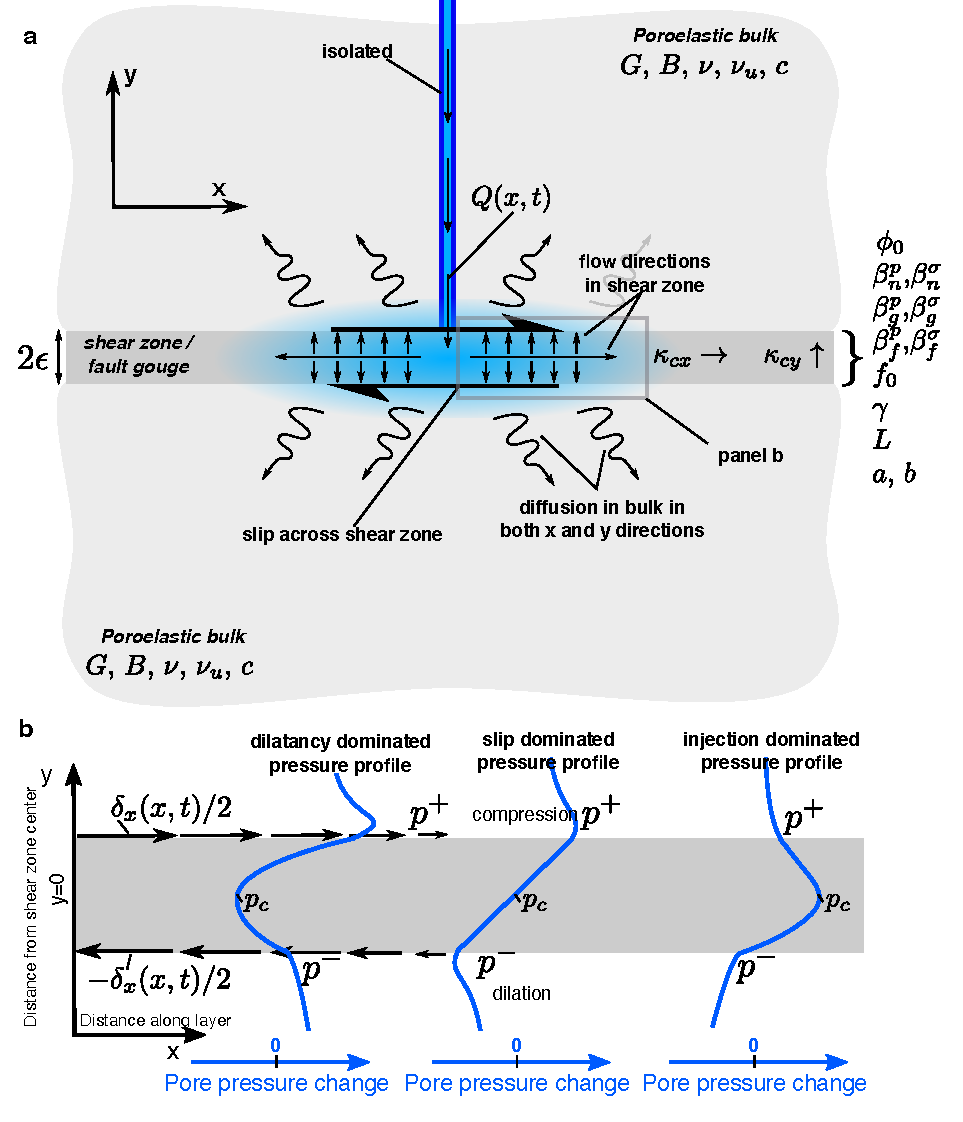
\includegraphics[scale = 0.85]{Figures/schema2.pdf} % this command will be ignored
\caption{Schematic overview of the problems setup and possible pore pressure profiles scenarios in the shear zone. {\bf a} Injection occurs in a thin shear zone embedded between two poroelastic solids of the same properties. This injection causes fluid migration along the shear zone, across the shear zone, and into the bulk. The evolving pore fluid pressure leads to slip across the shear zone. {\bf b} Pore pressure profiles that can occur during the propagation of a single rupture induced by injection. If the pore pressure diffusion is ahead of the rupture, then the shear zone has increased pressure at the center $p_c$ (right-most profile). Once considerable slip has occurred the inelastic dilatancy may have reduced the pressure, even to the point of being less than hydrostatic, which we may call a dilatancy dominated pore pressure (left-most profile). Between the two cases of an injection dominated regime and a dilatancy dominated regime we expect at or near the rupture tip the two effects may cancel. However, the compression and dilation of the host rock induced by the inhomogeneous slip can significantly change the pore pressures on either side of the shear zone ($p^+$ and $p^-$).}
\label{fig:schema}
\end{figure}

 A key question in induced seismicity is to understand when so-called runaway ruptures happen, that is ruptures that propagate well outside a pressurized region. This is a useful focal point to explain some of the general dynamics that we expect from the described problem above. When injection into a fault occurs, there are two important length scales along the $x$ dimension (Figure \ref{fig:schema}) that can interact and explain the dynamics of the slip. First, how far the pressure front from the injection site has diffused, which we can define as the region of significantly elevated pore pressure. Second, how far the rupture tip has propagated, which can be understood as the region of significant fault slip. If a fault has relatively low shear stress, i.e., its shear stress over initial effective normal stress is significantly below its reference friction coefficient, or is well-healed, which may be common in injection experiments, the pore pressure front controls how far the rupture tip can move since the frictional resistance is too great outside the pressure front \cite<e.g.,>{Larochelle2021}. However, if a fault is relatively well-stressed, or if the slipping region enters a more well-stressed portion of the fault or a portion of the fault with lower friction, then the rupture may become self-sustained and rupture outside the pressure front. Thus the rupture may initially be contained by the pressure front, but evolve to become a runaway rupture.

The interplay of the rupture tip and pressure front provides a useful qualitative explanation of the transition from a confined to runaway rupture. However, additional complexity,
which is related to the pressure profile across the fault, plays an important role in determining the if, when or how such a rupture can happen. If a rupture is initiated in a shear zone by injection, the pressure profile across the shear zone (i.e. pressure change with $y$, Figure \ref{fig:schema}{\bf b}) can be dominated by different mechanisms depending on whether observing the profile at a $x$ coordinate that is ahead of the rupture, at the tip or behind the tip (Figure \ref{fig:schema}b ). This will be particularly prominent for an in-plane rupture direction due to the volumetric straining of the bulk. If the pressurized zone is ahead of the rupture the shear zone central pressure ($p_c$) will be elevated. The pore pressures adjacent to the shear zone ($p^+$ and $p^-$) will also be elevated due to the leak-off into the bulk. Near the tip region, the influence of dilatancy has started to lower the pore pressure $p_c$, but furthermore volumetric straining of the bulk has caused an increase in pore pressure on the compressive side ($p^+$) and decrease on the dilating side ($p^-$) due to poroelastic coupling. Finally, behind the tip dilatancy may have further reduced the pressure $p_c$ and possibly reversed the sign compared to the background equilibrium pressure and caused flow back into the shear zone. We thus suggest that in order to model rupture propagation, earthquake nucleation, and understand runaway ruptures in a fluid-saturated medium due to injection, we must consider coupling that arises from the interplay of several mechanisms that alter the pore pressure.

\section{Governing equations} \label{sec:gov}
This section will describe the conservation laws, friction laws, and boundary conditions. All the governing equations and boundary conditions with the exception of Section \ref{sec:fluid}, which describes the fluid mass balance, are the same as in \citeA{Heimisson2021}. We state the equation with brief explanations for completeness, but refer the reader to \citeA{Heimisson2021} for more elaborate discussion and derivations.

\subsection{Poroelastic Bulk}

The quasi-static theory of poroelasticity can be described as four coupled partial differential equations written in terms of displacements $u_i$ and pressure changes $p$ relative to an equilibrium pressure state \cite<e.g.,>{Detournay1993,Cheng2016}

\begin{equation}
G  u_{i,kk} + \frac{G}{1-2\nu} u_{k,ki} = \alpha p_{,i}
\label{eq:G1}
\end{equation} 
and

\begin{equation}
\frac{1}{M} p_{,t} - \kappa p_{,kk} = - \alpha u_{k,kt},
\label{eq:G2}
\end{equation}
\noindent
where the material parameters are as follows: $G$: shear modulus, $\nu$: drained Poisson's ratio, $\alpha$: Biot-Willis parameter, $M$: Biot modulus, and $\kappa$ is the mobility  (the ratio between the permeability and fluid viscosity). In later expressions a different set of poroelastic material parameter may be used for compactness and increased intuition.

In this work, we assume plane strain deformation, in which case the governing equations can be reduced to three. Further simplification and decoupling of the governing equations is possible by using the McNamee-Gibson displacement functions \cite{Mcnamee1960,Verruijt1971}. In obtaining solutions to equations (\ref{eq:G1}) and (\ref{eq:G2}) we follow the strategy explained in the Appendix of \citeA{Heimisson2019} using the McNamee-Gibson displacement functions but using the boundary conditions listed in the next section.

\subsubsection{Boundary conditions} \label{sec:bc}

Here we apply the same boundary conditions as in \cite{Heimisson2021} at the interface, i.e. the shear zone and at infinity.

\begin{align}
& \lim_{y \rightarrow 0^\pm} u^+_x - u^-_x = \delta_x, \\
& \lim_{y \rightarrow 0^\pm} u^+_y - u^-_y = \delta_y, \\
& \lim_{y \rightarrow \pm \infty} u^\pm_x = 0 \text{ and } u^\pm_y = 0 , \\
& \lim_{y \rightarrow \pm \infty} p^\pm = 0, \\
& \lim_{y \rightarrow 0^\pm} \sigma^+_{xy} - \sigma^-_{xy} = 0, \\
& \lim_{y \rightarrow 0^\pm} \sigma^+_{yy} - \sigma^-_{yy} = 0,
\end{align}
where we have dropped the index notation and used $x$ and $y$ (as represented in Figure \ref{fig:schema}a).

The pore pressure in the shear zone is assumed to be bi-linear as in \citeA{Heimisson2021} This is a generalization of the leaky interface used in the plane strain dislocation solution of \citeA{Song2017}. The pore pressure across the shear zone is parameterized in terms of pressure at the center $p_c$ at $y=0$ and the pressure at the shear zone boundaries where the poroelastic bulk meets the shear zone, that is, $p^\pm$ at $y = \epsilon^\pm$. We can explicitly write out the assumed pore pressure profile as:

\begin{align}
    p(y) = & \frac{y}{\epsilon}(p^+ - p_c) + p_c \text{\quad if } 0 < y < \epsilon \nonumber \\ 
    p(y) = & \frac{y}{\epsilon}(p_c - p^-) + p_c \text{\quad if } - \epsilon < y < 0 .
    \label{eq:linear}
\end{align}
Thus equating the fluid mass flux into the shear zone and in the the bulk, and vice versa, gives rise to a pressure gradient boundary condition:

\begin{equation}
 \left. \frac{d p^\pm}{d y} \right|_{y = 0^\pm} = \pm \frac{\kappa_{cy}}{\kappa} \frac{(p^\pm - p_c)}{\epsilon},
 \label{eq:BC}
\end{equation}
where $\kappa_{cy}$ is the shear zone mobility in the $y$ direction and $\kappa$ is the poroelastic bulk mobility which is rated to the bulk hydraulic diffusivity by $c = M\kappa$. We note that boundary conditions for the bulk are applied at $y = 0^\pm$ but in the description of the shear zone we treat it as a finite layer with thickness between $y = \pm \epsilon$. This is because we take a boundary layer approach \cite<similar to Appedix B of>{Rudnicki2006} where the inner solution, the shear zone, is assumed to have a finite thickness. However, the outer solution, the bulk, approximates the layer as having an infinitesimal thickness. Thus the assumption that any variation along the length of the shear zone occurs over a length scale much smaller than $\epsilon$ is implicit. In other words, we always require that $\epsilon k \ll 1$, with $k$ representing the wavenumber (inverse of a wavelength) of any field that varies along the $x$-dimension.

\subsection{Frictional properties}

As in \citeA{Heimisson2021} we represent the frictional strength of the layer in an averaged sense.

Let us assume that the frictional strength of every point in the layer can be represented as follows:

\begin{equation}
\frac{\tau(x,t)}{\sigma(x,t) - p(x,y,t)} = f(x,y,t) \quad \text{ for } -\epsilon < y < \epsilon,
\label{eq:totforce}    
\end{equation}
where $\tau(x,t)$ is the sum of all contributions to the shear stress, both initial background value and slip contributions. We note that the shear stress is assumed to be spatially constant across the layer. Similarly, $\sigma(x,t)$ represents background initial effective normal stress (normal stress minus the ambient pore pressure) in addition to the slip induced changes in normal stress and we assume is spatially constant across the layer. However, we have separated from the description the perturbations in pore pressure $p(x,y,t)$ since, as previously discussed, they cannot be assumed to be constant in $y$. Using equation (\ref{eq:linear}) and averaging over the layer, we obtain:

\begin{equation}
\tau \frac{ ( p_c - p^+ ) \log \left( \frac{\sigma - p^-}{\sigma - p_c} \right) +  (p_c - p^- ) \log \left( \frac{\sigma - p^+}{\sigma - p_c} \right) }{2 (p_c - p^-) (p_c - p^+)} = \langle f \rangle ,
\label{eq:totforceave}    
\end{equation}
with the $\langle f \rangle$ representing the frictional coefficient of the layer. We have explored using the equation above for modeling the interface frictional strength, but we find that it renders very similar results as an linearized approximation valid in the limit of the pore pressure changes being small compared to the background normal stress:

\begin{equation}
  \tau = ({\sigma}- \langle p(t) \rangle  ) \langle f \rangle,
    \label{eq:RSFL}
\end{equation}
where $\langle p(t) \rangle$ is the average pressure across the layers and can be computed directly

\begin{equation}
    \langle p \rangle = \frac{1}{2 \epsilon} \int_{-\epsilon}^{\epsilon} p(y) dy = \frac{1}{2} \left( p_c  + \frac{p^+ + p^-}{2} \right).
    \label{eq:avep}
\end{equation}
Equation (\ref{eq:RSFL}) further offers a simpler interpretation of the role of the pore pressure in the effective normal stress compared to equation (\ref{eq:totforceave}), which helps in understanding the simulation results.

 We interpret the averaged friction coefficient $\langle f \rangle$ of the shear zone as being represented by the rate-and-state friction law \cite<e.g.,>{Dieterich1979,Ruina1983,Marone1998}:

\begin{equation}
  \langle f \rangle = \frac{1}{2 \epsilon} \int_{-\epsilon}^{\epsilon} f(x,y,t) d y = a \text{arcsinh} \left[ \frac{V}{2V_0} \exp \left(  \frac{f_0 + b \log (V_0 \theta/L)}{a} \right)   \right],
    \label{eq:avef}
\end{equation}
where we use the regularized form of the friction law that is also valid for slip speeds $V$ much smaller than the reference slip speed $V_0$ \cite{Rice1996,BenZion1997,Lapusta2000}. Here $a$ and $b$ are constitutive parameters that describe the rate dependence and state dependence of friction, respectively. Further, $f_0$ is the reference coefficient and $L$ is the characteristic slip distance over which the state evolves. The state variable is described by the aging law \cite{Ruina1983}:

\begin{equation}
    \frac{d \theta}{d t} =  1 - \frac{\theta V}{L} 
    \label{eq:aging}
\end{equation}

We note that here we have introduced a minor difference compared to \cite{Heimisson2021}. We represent friction using the regularized friction law whereas the non-regularized version was discussed by \cite{Heimisson2021}.  In the linearized analysis treated by \citeA{Heimisson2021}, there is no difference between the two versions.  

\subsection{Shear Zone}

Here we analyze the fluid and solid constituent mass balance of the shear zone gouge. This analysis is largely based on \citeA{Heimisson2021} although here we introduce new physical processes into fluid mass balance, which are detailed below. \citeA{Heimisson2021} linearized all relations around steady-state sliding, which is needed for the purpose of linearized stability analysis. While not strictly needed for a numerical algorithm, we will here also linearize and neglect non-linear terms that arise for various reasons. Firstly, this is done because we have adapted linear compressibility relationships, as is commonly done, for the fluid, solid and pore-space. Thus for consistency, all terms should be linearized. Second, some non-linear terms have a $\epsilon k$ scaling, which is by definition a small parameter. Third, since we adopt a boundary layer treatment of the shear zone with averaging in $y$ over the thickness of the layer, the non-linearity prevents such averaging from being carried out analytically and largely negates the computational benefits from the boundary layer treatment. 

\subsubsection{Fluid mass balance} \label{sec:fluid}


While other governing equations presented here are identical to those derived and used by \citeA{Heimisson2021}, we will introduce two additional physical processes to the fluid mass balance of the shear zone. We will thus re-derive the fluid mass balance. The two processes incorporate an injection or source term and allow for along shear zone lateral diffusion.

Within the shear zone, we state the fluid mass balance:

\begin{equation}
    \frac{\partial m}{\partial t} + \frac{\partial q_y}{\partial y} + \frac{\partial q_x}{\partial x}  = \frac{\partial}{\partial t} ( Q(x,t) ),
    \label{eq:cons}
\end{equation}
where $m$ is the fluid mass content and $q_y$ is fluid mass flux perpendicular to the fault (y-axis) and $q_x$ is the fluid mass flux parallel to the fault (x-axis). $Q(x,t)$ is the cumulative fluid mass injected per unit volume of the shear zone

We note that $m =  \rho_f n$, where $\rho_f$ is fluid density and $n = n^e + n^p$ is the sum of elastic and plastic void volume and thus

\begin{equation}
    \dot{m} = \dot{\rho}_f n + \rho_f \dot{n}.
    \label{eq:dotm}
\end{equation}
Following \citeA{Heimisson2021} we linearize $\dot{n}^e = \phi (\beta_n^p \dot{p} - \beta_n^{\sigma} \dot{\sigma} )$ and $\dot{\rho}_f = \rho_{fo}(\beta_f^p \dot{p} + \beta_f^\sigma \dot{\sigma} )$, where $\beta_f^p$ and $\beta_n^p$ are fluid and elastic void compressibilities respectively and $\sigma > 0$ means increased compression, also know as ``the compression positive'' convention. The reference compressibilities are defined at the reference void volume fraction $\phi$ and fluid density $\rho_{fo}$. We assume the reference void volume fraction is the same as the porosity. Similarly, we assume plastic void fraction is equal to the plastic porosity: $n^{pl} = \phi^{pl}$. Thus equation (\ref{eq:dotm}) becomes: 

\begin{equation}
    \dot{m} = \rho_{fo} \phi (\beta_f^p \dot{p} + \beta_f^\sigma \dot{\sigma} ) + \rho_{fo} \phi (\beta_n^p \dot{p} - \beta_n^{\sigma} \dot{\sigma} + \dot{\phi}^{pl}/\phi ).
    \label{eq:mdot}
\end{equation}
Darcy's law provides the following linearization:

\begin{equation}
    q_x =   - \rho_{fo} \kappa_{cx}\frac{\partial p}{\partial x}
    \label{eq:Darcyx}
\end{equation}
where $\kappa_{cx}$ is the mobility (permeability over dynamic viscosity) for fluid flux along the x-axis within the shear zone and is assumed to be spatially constant with respect to $x$.

Combining equations (\ref{eq:cons}), (\ref{eq:mdot}), and (\ref{eq:Darcyx}) and integrating with respect to the y-axis gives

\begin{equation}
    2 \epsilon \rho_{fo} \phi \left[ (\beta_f^p + \beta_n^p ) \langle \dot{p} \rangle + (\beta_f^\sigma - \beta_n^{\sigma}) \dot{\sigma} + \langle \dot{\phi} \rangle^{pl}/\phi ) \right] + q_y^+ - q_y^- - 2 \epsilon \rho_{fo} \kappa_{cx} \frac{\partial^2 \langle p \rangle}{\partial x^2}  = 2 \epsilon \dot{Q}(x,t)
\end{equation}
where the source terms $Q$ is assumed constant with respect to $y$. 

Inserting for the fluid mass flux in $y$ direction given a linear pressure distribution in the shear zone (equations (\ref{eq:BC}) and (\ref{eq:linear})) provides:

\begin{equation}
      \langle \dot{p} \rangle + \frac{\beta_f^\sigma - \beta_n^{\sigma}}{\beta_f^p + \beta_n^p } \dot{\sigma}    =  - \frac{\langle \dot{\phi} \rangle^{pl}}{\phi (\beta_f^p + \beta_n^p )} + \frac{\kappa_{cy}}{\epsilon^2 \phi(\beta_f^p + \beta_n^p )} (\frac{1}{2}(p^+ + p^-) - p_c) + \frac{\kappa_{cx}}{\phi(\beta_f^p + \beta_n^p) } \frac{\partial^2 \langle p \rangle}{\partial x^2} + \frac{\dot{Q}(x,t)}{\rho_{fo}\phi(\beta_f^p + \beta_n^p)}.
     \label{eq:pc}
\end{equation}	
We have thus derived an equation that relates average pressure, normal stress, dilatancy, along shear zone diffusion, and fluid mass injection. The inelastic changes in porosity $\phi^{pl}$ is taken as

\begin{equation}
    \langle \phi \rangle^{pl} = \phi_0^{pl} -  \gamma \log \left( \frac{V_0 \theta}{L} \right),
    \label{eq:phidil}
\end{equation}
based on \citeA{Segall1995} and \citeA{Segall2010b}, which proposed that the inelastic porosity is a function of the frictional state variable $\phi^{pl} (\theta)$. Recently this idea has gained more observational support \cite{Proctor2020}. Further, we assume that the frictional state variable $\theta$ describes the average porosity change in the shear layer. 

Before implementing equation (\ref{eq:pc}) numerically, we analytically integrate to obtain

\begin{equation}
      \langle {p} \rangle + \frac{\beta_f^\sigma - \beta_n^{\sigma}}{\beta_f^p + \beta_n^p } {\sigma}    = \frac{1}{\phi(\beta_f^p + \beta_n^p)} \left( \frac{{Q}(x,t)}{\rho_{fo}}  - \langle {\phi} \rangle^{pl} +  \int_0^t \frac{\kappa_{cy}}{\epsilon^2} (\frac{1}{2}(p^+ + p^-) - p_c) + \kappa_{cx} \frac{\partial^2 \langle p \rangle}{\partial x^2} dt' \right),
     \label{eq:pcI}
\end{equation}	
where it is assumed that all fields are 0 at $t=0$

\subsubsection{Solid gouge constituent mass balance}

We use the same solid constituent mass balance as in \citeA{Heimisson2021} to obtain a constitutive relationship for fault perpendicular displacements:

\begin{equation}
     \dot{\delta}_y =  2 \epsilon \left( \frac{ \phi }{1 - \phi} \beta_n^p - \beta_g^p \right) \left[  \langle \dot{p} \rangle  - \frac{ \left( \frac{ \phi }{1 - \phi} \beta_n^{\sigma}  +    \beta_g^\sigma \right)}{\left( \frac{ \phi }{1 - \phi} \beta_n^p - \beta_g^p \right)} \dot{\sigma}  \right] + 2 \epsilon \frac{ \langle \dot{\phi} \rangle^{pl}}{1 - \phi}.
\end{equation}
Assuming that at $t=0$ the fault is in pressure equilibrium and steady-state sliding, such that no net dilatancy or compaction occurs, then the equation can be integrated

\begin{equation}
     {\delta}_y =  2 \epsilon \left( \frac{ \phi }{1 - \phi} \beta_n^p - \beta_g^p \right) \left[  \langle {p} \rangle  - \frac{ \left( \frac{ \phi }{1 - \phi} \beta_n^{\sigma}  +    \beta_g^\sigma \right)}{\left( \frac{ \phi }{1 - \phi} \beta_n^p - \beta_g^p \right)} {\sigma}  \right] + 2 \epsilon \frac{ \langle {\phi} \rangle^{pl}}{1 - \phi}.
     \label{eq:dy}
\end{equation}



\section{Solutions for Coupled Shear Zone and Bulk} \label{sec:porosol}

In this section we define the joint Fourier-Laplace transform 

\begin{equation}
\bar{\hat{\delta}}_x(s,k) = \int_{0}^{\infty} \int_{-\infty}^{\infty} \delta_x(t,x)
e^{-ikx-st} dx dt ,
\label{eq:LF}
\end{equation}
applied here in the slip $\delta_x(x,t)$, or displacement discontinuity across the layer in the $x$ direction, where the bar symbol represents the Laplace transform in time and the hat the Fourier transform along the $x$ spatial axis. Some symbols may not carry the hat symbol if they are explicitly written out in term in terms of the wavenumber $k$.
	
As in \citeA{Heimisson2021}, we follow the procedure outlined by \citeA{Heimisson2019}. In particular, we derive solutions in the Fourier-Laplace domain for shear stress, pore pressure, and normal stress change at the slip surface ($y \rightarrow 0^\pm$). As provided by \citeA{Heimisson2021} the relationships between change in shear stress $\bar{\hat{\tau}}'$, pore pressure change on either side of the layer $\bar{\hat{p}}^\pm$, and change in total normal stress $\bar{\hat{\sigma}}_{yy}$ in terms of $\bar{\hat{\delta}}_x$, $\bar{\hat{\delta}}_y$, and $\bar{\hat{p}}_c$ are given by the following equations:
	
\begin{equation}
\bar{\hat{\tau}} = -  \frac{G |k| \bar{\hat{\delta}}_x}{2(1-\nu_u)} \bar{H}_1(s,k)
\label{eq:tau}
\end{equation}
and

\begin{equation}
\bar{\hat{p}}^\pm = \mp \frac{ik G B \bar{\hat{\delta}}_x}{3} \frac{1+\nu_u}{1-\nu_u} \bar{H}_2(s,k) -  \bar{\hat{p}}_c \frac{\mathcal{F}}{\mathcal{F} + 1} \left( \bar{H}_2(s,k) - 1 \right) + \frac{|k| G B \bar{\hat{\delta}}_y}{3} \frac{1+\nu_u}{1-\nu_u} \bar{H}_2(s,k) ,
\label{eq:p}
\end{equation}
and

\begin{equation}
\bar{\hat{\sigma}}_{yy} = \bar{\hat{p}}_c \frac{3 }{2 B (1 + \nu_u)} \frac{ \mathcal{F} }{\mathcal{F} + 1} (\bar{H}_1(s,k) - 1) - \frac{G |k| \bar{\hat{\delta}}_y}{2(1-\nu_u)} \bar{H}_1(s,k),
\label{eq:sigyy}
\end{equation}
where

\begin{equation}
\bar{H}_1(s,k) = 1 - \frac{2(\nu_u - \nu)}{1-\nu} \frac{c k^2}{s} \frac{1 + \mathcal{F}}{\mathcal{F} + \sqrt{1+s/c k^2}}\left( \sqrt{1+s/c k^2} - 1 \right),
\label{eq:H1}
\end{equation}
and

\begin{equation}
\bar{H}_2(s,k) = \frac{\sqrt{1+s/c k^2} - 1}{\sqrt{1+s/c k^2} + \mathcal{F}} .
\label{eq:H2}
\end{equation}
$\mathcal{F}$ is a dimensionless group that characterizes the importance of flux across the fault:

\begin{equation}
\mathcal{F} = \frac{\kappa_{cy}}{\kappa} \frac{1}{|k|\epsilon} .
\label{eq:F}
\end{equation}

We now seek to invert the Laplace transform. We define

\begin{equation}
    \bar{K}_1 = \bar{H}_1 - 1 \text{ and } \bar{K}_2 = \bar{H}_2 - 1.
\end{equation}
As was shown by \citeA{Heimisson2019}, $\bar{H}_1$ and $\bar{H}_2$ approach unity in the limit of short time or negligible diffusion, which reduces Eqs. (\ref{eq:tau}), (\ref{eq:p}), and (\ref{eq:sigyy}) to their corresponding undrained limits. $\bar{K}_1$ and $\bar{K}_2$ thus represent the transient changes in shear stress and pore pressure on the fault that arise due to pore pressure diffusion.

We note that $\bar{H}_1 = 1 - 2 (\nu_u - \nu)/(1 - \nu) (1 + \mathcal{F}) (c k^2/s) \bar{H}_2$. Thus in the time domain the inverse transform of $\bar{H}_1$ is closely related to the time integral of the inverse transform of $\bar{H}_2$. Using the convolution theorem for Laplace transforms we find that Eqs. (\ref{eq:tau}) and (\ref{eq:p}) take the form:

\begin{equation}
\hat{\tau}' = -  \frac{G |k|}{2(1-\nu_u)} \left( \hat{\delta}_x + \int_0^t \hat{\delta}_x(t') K_1 (t - t',k) dt' \right),
\label{eq:tauIL}
\end{equation}	


\begin{align}
\hat{p}^\pm = & \mp \frac{ik  G B }{3} \frac{1+\nu_u}{1-\nu_u} \left( \hat{\delta}_x + \int_0^t \hat{\delta}_x(t') K_2 (t - t',k) dt' \right) - \frac{\mathcal{F}}{\mathcal{F} + 1} \int_0^t \hat{p}_c(t') K_2 (t - t',k) dt' \label{eq:pIL} \\ \nonumber
& + \frac{|k| G B }{3} \frac{1+\nu_u}{1-\nu_u} \left( \hat{\delta}_y + \int_0^t \hat{\delta}_y(t') K_2 (t - t',k) dt' \right).
\end{align}	

 and
 
\begin{equation}
\hat{\sigma}_{yy} = \frac{3 }{2 B (1 + \nu_u)} \frac{  \mathcal{F} }{\mathcal{F} + 1} \int_0^t \hat{p}_c(t') K_1(t-t',k) dt' - \frac{G |k| }{2(1-\nu_u)} \left( \hat{\delta}_y + \int_0^t \hat{\delta}_y(t') K_1 (t - t',k) dt' \right)
\label{eq:sigyyIL}
\end{equation}

We have thus separated the undrained response and the transient diffusion behavior. This behavior  characterized by the convolution kernels $K_1$ and $K_2$ that represent the inverse Laplace transforms of $K_1$ and $K_2$ respectively. In other words $K_1(t) =  \mathcal{L}^{-1} \left\{ \bar{K}_1 \right\} (t)$ and $K_2(t) =  \mathcal{L}^{-1} \left\{ \bar{K}_2 \right\} (t)$.

Analytical expressions for $K_1$ and $K_2$ can be attained through repeated application of the convolution theorem to separate $\bar{K}_1$ and $\bar{K}_2$ into factors of known inverse Laplace transforms.

\begin{align}
 K_1(t,k) & =  - \frac{2 (\nu_u - \nu)}{1-\nu} c k^2 (1 + \mathcal{F}) \left( 1 + \frac{1}{\mathcal{F} - 1} \left[ \mathcal{F} e^{ (\mathcal{F}^2-1)c k^2 t } \text{erfc}\left( \mathcal{F}\sqrt{c k^2 t } \right) - \mathcal{F}  + \text{erf} \left( \sqrt{c k^2 t } \right)  \right]   \right) \label{eq:K1}  \\ 
K_2(t,k) & =  - c k^2 (1 + \mathcal{F}) \left[ \frac{e^{-c k^2 t}}{\sqrt{\pi c k^2 t}} - \mathcal{F} e^{ (\mathcal{F}^2-1)c k^2 t } \text{erfc}\left( \mathcal{F}\sqrt{c k^2 t } \right)  \right]  \label{eq:K2}    .
\end{align}	
We note that kernel $K_2$ is singular when $t \rightarrow 0$. However, this is an integrable singularity and the convolution kernel can be integrated in the sense of taking a Cauchy principal value.

In summary, equations (\ref{eq:tauIL}), (\ref{eq:pIL}), and (\ref{eq:sigyyIL}) represent analytical solutions for the shear stress, pore pressure (at shear zone boundary), and normal stress given a time-history of slip $\delta_x$, opening $\delta_y$ and/or shear zone center pore pressure $p_c$ which have been transformed in the wavenumber (Fourier) domain. Alternatively, these expressions represent analytical solutions for a single plane wave perturbation in slip $\delta_x$, $\delta_y$ and/or $p_c$ of generic form $f(t)\exp(ikx)$, where $f(t)$ is some time-dependent function. In section \ref{sec:Fser} we use this property to construct general solutions for arbitrary histories of slip $\delta_x$, opening $\delta_y$ and/or shear zone center pore pressure $p_c$.

\section{Numerical Method} \label{sec:num}

\subsection{Fourier series representation of poroelastic relations}	\label{sec:Fser}

We represent $\delta_x$, $\delta_y$ and $p_c$ as a Fourier series

\begin{equation}
    \delta_x (x,t) = \sum_{n = -N/2}^{N/2 - 1} D_{x,n}(t) e^{ik_n x}, \quad k_n = \frac{2 \pi n}{\lambda},
\end{equation}

\begin{equation}
    \delta_y (x,t) = \sum_{n = -N/2}^{N/2 - 1} D_{y,n}(t) e^{ik_n x}, \quad k_n = \frac{2 \pi n}{\lambda},
\end{equation}

and
\begin{equation}
    p_c(x,t) = \sum_{n = -N/2}^{N/2 - 1} P_n(t) e^{ik_n x}, \quad k_n = \frac{2 \pi n}{\lambda},
\end{equation}
where $N$ is even and equal to the number of points at which $\delta(x,t)$ and $p_c(x,t)$ are evaluated, $\lambda$ represents the length of the simulation domain. The Fourier transform is given by 

\begin{equation}
    \hat{\delta}_x(k,t) = \sum_{n = -N/2}^{N/2 - 1} 2 \pi D_{x,n}(t) \delta_D(k - k_n),
\end{equation}
and corresponding relations exist for $\hat{p}_c$ and $\hat{\delta}_y$ where $\delta_D$ is the Dirac delta function. Inserting the transformed series into equations (\ref{eq:tauIL}), (\ref{eq:pIL}) , and (\ref{eq:sigyyIL}) and performing the trivial inverse Fourier transforms provide

\begin{equation}
\tau' = -  \frac{G}{2(1-\nu_u)}  \sum_{n = -N/2}^{N/2 - 1}   |k_n| \left(D_{x,n}(t) + \int_0^t D_{x,n}(t') K_1 (t - t',k_n) dt' \right) e^{ik_n x},
\label{eq:tauS}
\end{equation}	

\begin{align}
p^\pm =   \sum_{n = -N/2}^{N/2 - 1}  \bigg( \mp & \frac{i G B }{3} \frac{1+\nu_u}{1-\nu_u} k_n \left[ D_{x,n}(t) + \int_0^t D_{x,n}(t') K_2 (t - t',k_n) dt' \right] + \ldots \nonumber \\ 
 & \frac{G B }{3} \frac{1+\nu_u}{1-\nu_u} |k_n| \left[ D_{y,n}(t) + \int_0^t D_{y,n}(t') K_2 (t - t',k_n) dt'  \right] - \dots \nonumber  \\ 
& \left. \frac{  \mathcal{F}(k_n) }{\mathcal{F}(k_n) + 1} \int_0^t P_n(t') K_2 (t - t',k_n) dt'    \right) e^{ik_n x} ,
\label{eq:pS}
\end{align}	
and

\begin{align}
\sigma_{yy} = \frac{3 }{2 B (1 + \nu_u)} \sum_{n = -N/2}^{N/2 - 1} \left( \frac{  \mathcal{F}(k_n) }{\mathcal{F}(k_n) + 1}  \int_0^t P_n(t') K_1(t-t',k_n) dt' \right. - \ldots \nonumber  \\
\left. \frac{G}{2(1-\nu_u)} |k_n| \left[D_{y,n}(t) + \int_0^t D_{y,n}(t') K_1 (t - t',k_n) dt'\right]  \right) e^{ik_n x}
\label{eq:sigyyS}
\end{align}
	
Testing and validation revealed that the first term of the pore pressure (Eq. \ref{eq:pS}) is prone to developing the Gibbs phenomenon in the presence of steep gradients. This may stem from  how the sign of the pore pressure depends on $k_n$ and not the absolute value of $|k_n|$ as for other terms. Oscillations, such as the Gibbs phenomena, are somewhat mitigated by the diffusional nature of the pore pressure where short-wavelength oscillations diffuse rapidly. However, a much improved convergence of the series in Eq. (\ref{eq:p}) and nearly complete removal of the Gibbs phenomenon can be achieved with a Lanczos sigma factor \cite{Duchon1979}:

\begin{align}
\label{eq:pSLanc}
p^\pm =   \sum_{n = -N/2}^{N/2 - 1}  \bigg( \mp & \frac{i G B }{3} \frac{1+\nu_u}{1-\nu_u} k_n \text{ sinc} \left( \frac{n}{N/2} \right)  \left[ D_{x,n}(t) + \int_0^t D_{x,n}(t') K_2 (t - t',k_n) dt' \right] + \ldots \nonumber \\ 
 & \frac{G B }{3} \frac{1+\nu_u}{1-\nu_u} |k_n| \left[ D_{y,n}(t) + \int_0^t D_{y,n}(t') K_2 (t - t',k_n) dt' \right] - \dots \nonumber  \\ 
& \left. \frac{  \mathcal{F}(k_n) }{\mathcal{F}(k_n) + 1} \int_0^t P_n(t') K_2 (t - t',k_n) dt'    \right) e^{ik_n x} ,
\end{align}	
where $\text{sinc}(x) = \sin{ (\pi x)}/(\pi x)$ is the normalized sinc function. It is worth noting that an inverse FFT of the Fourier coefficients in equations \ref{eq:tauS}, \ref{eq:pS}, \ref{eq:sigyyS}, and \ref{eq:pSLanc}  is an efficient way to compute the stresses and pore pressure at each value of $x$.

\subsubsection{Comparison to Song and Rudnicki (2017)}
To partially validate solutions in the previous section we compare to the analytical solution provided for a single edge dislocation on a leaky plane provided by \citeA{Song2017} (Figure \ref{fig:Song}). In the problem analyzed by \citeA{Song2017} $\delta_x = \mathcal{H}(t)\mathcal{H}(-x)$, $\delta_y = 0$, $p_c = 0$, in which case $\sigma_{yy} = 0$. We use equations (\ref{eq:tauS}) and (\ref{eq:pSLanc}) after retrieving Fourier series coefficients using a fast Fourier transform (FFT) algorithm of $\delta_x = \mathcal{H}(t)\mathcal{H}(-x)$ evaluated on a domain size ranging from $x = -50$ to $x = 50$ m. Comparison in Figure \ref{fig:Song} reveals excellent agreement between the two approaches.

\begin{figure}[H]
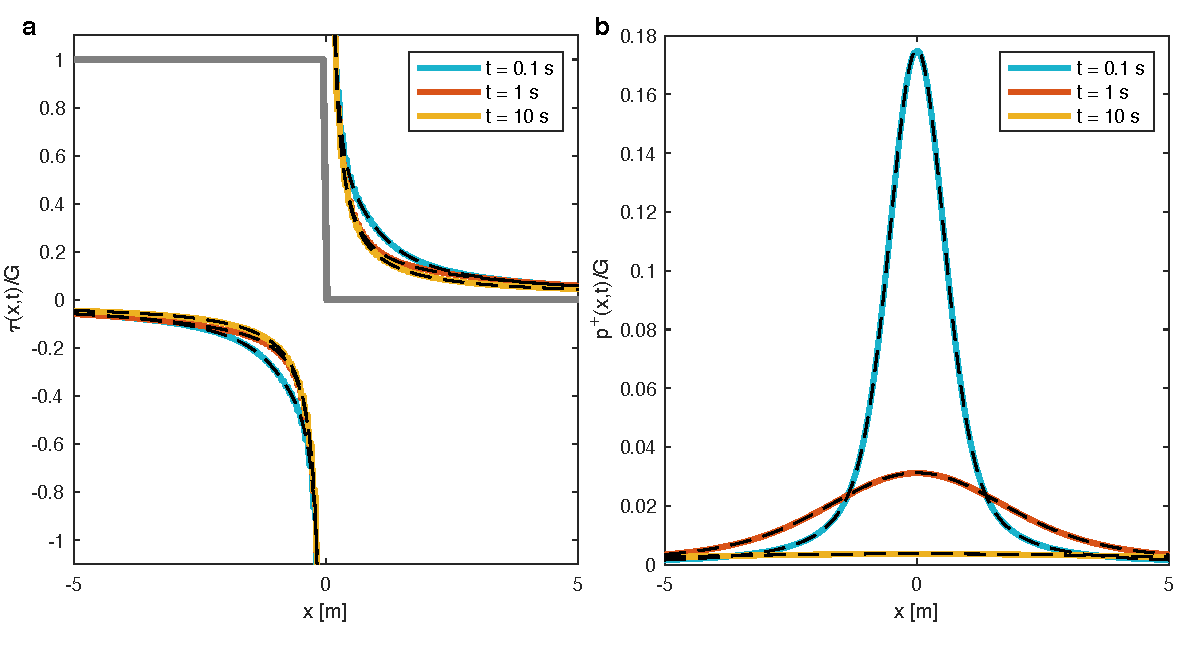
\includegraphics[scale = 0.8]{Figures/Pore_pressure_benchmark_SandR2017.pdf} % this command will be ignored
\caption{Comparison of equations (\ref{eq:tauS}) and (\ref{eq:pSLanc}) to equations (A1) and (72) respectively in \citeA{Song2017}. Colored lines represent the spectral boundar-integral solution and overlapping dashed black lines represent the \citeA{Song2017} solution. \textbf{a} Shear stress normalized by shear modulus $G$ near the dislocation edge (indicated in gray) of unit slip amplitude at three different times, which span approximately the undrained, drained limits as well as an intermediate stage. \textbf{b} pore pressure due to the same edge dislocation. Results are shown for $c = 1$ m$^2$/s, $B = 0.5$, $\kappa_c/(\kappa \epsilon) = 1 $ m$^{-1}$, $\nu=0.15$, $\nu_u = 0.45$.}
\label{fig:Song}
\end{figure}

\subsection{Time-stepping} \label{sec:time}

Here we describe the time-stepping scheme to simulate slow and fast slip with dilatancy and fluid injection into the faults. The scheme builds on the predictor-corrector schemes of \citeA{Lapusta2000} and \citeA{Heimisson2020}.  However, several significant modifications have been introduced to resolve fluid diffusion. Below we shall describe the stages of a single time-step by the algorithm. We also refer the reader to the source code \cite{elias_rafn_heimisson_Poro_SBIM} for a more explicit implementation of the time-stepping scheme. 
\begin{enumerate}

\item Initial explicit Euler prediction is made for time $t^{n+1} = t^n + \Delta t$ for $\delta_x^*$, $\delta_y^*$, $p_c^*$, $V^*$, where the asterisk represents the prediction of the next time-step.

\item Fourier coefficients are computed corresponding to the prediction values $\delta_x^*$, $\delta_y^*$, $p_c^*$, that is $D_{x,n}^*$, $D_{y,n}^*$, $P_{n}^*$ using a Fast-Fourier Transform (FFT).

\item Using equations (\ref{eq:tauS}), (\ref{eq:sigyyS}), and (\ref{eq:pSLanc}) the Fourier coefficients for changes in shear stress, normal stress and boundary pore pressure are computed and an inverse FFT is used to sum all Fourier modes.

\item Prediction for shear stress $\tau^*$ and effective normal stress $(\sigma - p)^*$ is computed. In the results, we use the average pore pressure $\langle p \rangle$; however, we note that $p$ could here represent any number of pore pressure values, e.g. $p^\pm$ or $p_c$, depending on what assumptions are made about the relevant pore pressure in the shear localization region. In our numerical implementation \cite{elias_rafn_heimisson_Poro_SBIM}, the user sets which pore pressure to use.

\item Prediction of the updated state-variable is computed using the analytical integration of the aging law by \citeA{Kaneko2011} which is assumes constant slip speed from $t$ to $t + \Delta t$ 

\begin{equation}
    \theta^* = \theta^p \exp \left( - \frac{\Delta t}{2 L} (V^n + V^*)  \right) + \frac{2 L}{(V^n + V^*)} \left( 1 - \exp \left( - \frac{\Delta t}{2 L} (V^n + V^*)  \right)  \right),
\end{equation}
where we have taken taken the slip speed as the average $(V^p + V^*)/2$ between the slip speed at time $t^n$ and $t^{n+1} = t^n + \Delta t$. Here we use the superscript $^n$ to represent the fields at the previous time step, that is at time $t^n$.

\item Via an algebraic manipulation of the rate-and-state friction law (\ref{eq:RSFL}) and (\ref{eq:avef}) a correction for the slip speed is computed
\begin{equation}
    {V}^{**} = 2 V_0 \sinh \left( \frac{{\tau}^* - \eta V^*}{a (\sigma - p)^*} \exp \left( - f_0/a - \frac{b}{a}\log(V_0 {\theta}^*/L) \right) \right).
    \label{eq:FLn}
\end{equation}

However, for locations along the fault where the slip speed exceeds a threshold value (here set to 1 cm/s) the previous expression is found to lead to numerical dispersion and the slip speed is obtained by solving the following non-linear equation as done by \citeA{Heimisson2020}:
 
 \begin{equation}
    \left|     {V}^{**} - 2 V_0 \sinh \left( \frac{{\tau}^* - \eta V^*}{a (\sigma - p)^*} \exp \left( - f_0/a - \frac{b}{a}\log(V_0 {\theta}^*/L) \right) \right) \right| = 0 .
    \label{eq:FLnim}
\end{equation}


\item Using the new slip speed correction $V^{**}$ the state variable is also updated

\begin{equation}
    \theta^{**} = \theta^p \exp \left( - \frac{\Delta t}{2 L} (V^n + V^{**})  \right) + \frac{2 L}{(V^n + V^{**})} \left( 1 - \exp \left( - \frac{\Delta t}{2 L} (V^n + V^{**})  \right)  \right),
\end{equation}
and from equation (\ref{eq:phidil}) $\langle \phi \rangle_{pl}^{**}$ is computed using $\theta^{**}$.

\item Updating $p_c$: for the sake of brevity, we will only refer to the code \cite{elias_rafn_heimisson_Poro_SBIM}, see also data availability statement, for a detailed implementation of this time-step, but a summary follows. In equation (\ref{eq:pcI}) (after substituting with equation (\ref{eq:avep}) for $\langle p \rangle$) we approximate the $\partial^2/\partial x^2$ derivative with second-order finite difference approximation. The time-integral is discretized using a trapezoidal rule. Predictions from step 1 and 3 are used to compute the various fields at time $t^{n+1}$ except we solve for $p_c^{**}$ (the prediction of $p_c$ for time $t^{n+1}$) implicitly by solving a system of linear equations. 

\item Finally $p_c^{**}$ is used to update $\delta_{y}^{**}$, $\langle p \rangle ^{**}$, and $\delta_x^{**} = \delta_x^{n} + \Delta t (V^n + V^{**})/2$.

\end{enumerate}

After the steps above, the algorithm determines if it will proceed to the next time-step or reiterate following these rules.

\begin{itemize}

    \item A minimum of one iteration is used. If the algorithm finishes the aforementioned steps for the first time at the current time then it must iterate again. The algorithm moves back to step 1, but instead of explicit guesses for the new time step it uses previous updates. That is $\delta_x^{**} \rightarrow \delta_x^{*}$, $\delta_y^{**} \rightarrow \delta_y^{*}$, and $p_c^{**} \rightarrow p_c^{*}$.
    \item If a minimum one iteration has been done, the algorithm checks for absolute and relative error in the estimate of $p_c$. That is if $\text{max} (|p_c^{**} - p_c^*|)/(a \sigma_0) > \xi/10$ (where $a$ is the direct effect parameter)  or $||p_c^{**} - p_c^*||_1/||p_c||_1 > \xi/10$ is violated then a new time-step is selected $\Delta t \rightarrow \Delta t /2$ and the algorithm proceeds to step 1 using the following initial predictions $(\delta_x^{**} + \delta_x^{n})/2 \rightarrow \delta_x^{*}$, $(\delta_y^{**} + \delta_y^{n})/2 \rightarrow \delta_y^{*}$, and $(p_c^{**} + p_c^n)/2 \rightarrow p_c^{*}$. Here $\xi$ is a factor that controls the accuracy of the solution, in simulations shown later this is set to $\xi = 1/32$, see Appendix B for more discussion of $\xi$.
    \item If both a minimum of one iteration has been carried out and the error tolerances are satisfied, the algorithm proceeds to a new time step and $^{**}$ predictions are assigned as field values are time $t^{n+1}$. Finally, the new initial time-step is selected $\Delta t \rightarrow \text{min} (\xi V^{n+1}/L , 1.1 \cdot \Delta t )$ where first we make sure that the state evolution is well resolved, by picking $\xi$ sufficiently small. Second, we make sure not to grow the time-step too much if the pore pressure evolution requires a smaller time-step than indicated by $\xi V^{n+1}/L$.
\end{itemize}


\subsection{Convolution kernel computation and truncation}

Alongside with the time stepping, which was described in the previous section, we update and calculate the convolution in equations (\ref{eq:tauS}), (\ref{eq:sigyyS}), and (\ref{eq:pSLanc}). In computing the convolution we first compute a kernel values at lag times $t_i$ for each wavenumber $k_n$ i.e. $K_1(t_i,k_n)$ and $K_2(t_i,k_n)$, where $t_i$ is selected to span a time interval from $\zeta_l \text{min} (t_b, t_f)$ to $\zeta_u \text{min} (t_b, t_f)$. In practice we take $\zeta_l = 10^{-6}$ and $\zeta_u = 20$ and $t_b$ and $t_f$ are the diffusion time-scales of the bulk and of the flux through the shear zone:

\begin{equation}
    t_{b} = \frac{1}{c k^2},
    \label{eq:tb}
\end{equation}
 and
 
\begin{equation}
    t_{f} = \frac{1}{\mathcal{F}^2 c k^2} = \frac{\kappa^2 \epsilon^2}{\kappa_c^2 c }.
    \label{eq:tf}
\end{equation}

We thus evaluate the convolution kernels between a time that is negligible compared to the diffusional time-scales $\zeta_l \text{min} (t_b, t_f)$, up to a time that is long compared to the diffusional time scales $\zeta_u \text{min} (t_b, t_f)$. Evaluation points $t_i$ are selected by combining both points at a linearly equally spaced times, and logarithmically equally spaced times. Here we use 1024 evaluation points, but we found for in some cases, such as the benchmarking against the linear stability analysis of \citeA {Heimisson2021} that much fewer evaluation points were needed.

Since we pre-compute the convolution kernels we need to determine the values of the Fourier coefficients $D_{x,n}$, $D_{y,n}$, $P_{n}$ at times $t-t_i$. This is done by storing the Fourier coefficients' values at selected times and then determining their values at the convolution times $t_i$ by linear interpolation. 

The criteria for storing a Fourier coefficient value are implemented by setting an integer $N_{st}$, which is the maximum number of time-steps that can be taken without storing the Fourier coefficients. We compute 

\begin{equation}
   N_{st} = \left \lfloor \min ( 1 + \min(t_f,t_b)/ \Delta t ; 1 + \min(a  \sigma_0 / (p_c^n - p_c^{lst} ) )/20;  N_{st}^{\max}  ) \right \rfloor,
\end{equation}
where $p_c^{lst}$ is the vector of $p_c$ values when the Fourier coefficients were last stored and  $N_{st}^{\max}$ is some user-determined value that makes sure the coefficients are sampled at least every $N_{st}^{\max}$ time-step. The first criterion in the equation makes sure that the minimum diffusion time is resolved in the stored Fourier coefficients and thus changes the Fourier coefficients that occur on time scales relevant for diffusion are stored. Testing has suggested that under-sampling here may not be an issue since the shortest diffusion times correspond to the largest wavenumbers (shortest wavelengths) and if the simulation is well resolved, then the influence of these wavelengths is negligible. The second criterion makes sure that if the pore pressure is changing rapidly, then information of these rapid changes is stored in the stored coefficients. This is particularly important for injection problems. However, for efficiency we overwrite the value above for $N_{st}$ if $t^n - t^{lst} < \zeta_l \text{min} (t_b, t_f)$, where $t^{lst}$ is the time when the coefficients were last stored, in which case we set $N_{st} = N_{st}^{\max}$. This makes sure that we do not store coefficients over time scales too short for any diffusional process to occur. This makes the seismic phase of the simulations much more efficient. 

\section{Application} \label{sec:app}

Here we show an application of the code. We compare the code to the \citeA{Guglielmi2015} experiment, in which fluid was injected into a shallow fault and slip and pressure were monitored. The slip and pressure data was previously analyzed by \citeA{Larochelle2021} by modeling 1D diffusion in a plane strain linear elastic bulk with rate-and-state friction. We use their parameter estimates (see also table \ref{symbolstable}) and their simplified pore pressure history \cite<see Figure 2 in>{Larochelle2021} as input, but we vary other processes and parameters that were not accounted for by \citeA{Larochelle2021}, or in most comparable studies, such as dilatancy, different permeabilities of the bulk compared to the shear zone, and poroelastic parameters. Specifically, we explore a set of parameters where the dilatancy coefficient takes values $\gamma = $0 , 1.7$\cdot$10$^{-5}$, and 1.7$\cdot$10$^{-4}$. Further, the bulk hydraulic diffusivity is $c = 4\cdot$10$^{-8}$ or 4$\cdot$10$^{-7}$ m$^2$/s and the undrained Poisson's ratio is $\nu = $0.35 or 0.262. We note further discussion of parameters in Appendix A.

We follow the setup and initial conditions as implemented by \citeA{Larochelle2021}. However, some critical differences in model setup and characterization of fluid flow are worth mentioning.  \citeA{Larochelle2021} implement 1D isotropic diffusion, meaning the pressure in the bulk and shear zone is spatially constant in $y$, and no fluid-solid coupling of the bulk. This implies isotropic diffusivity across the shear zone and bulk and that the bulk is purely elastic, thus no coupling of fluid flow and deformation. Here we can create an elastic bulk response by selecting the hydraulic diffusivity as either very large or very small (drained and undrained conditions, respectively). However, this would make the bulk extremely diffusive or impermeable, which is then inconsistent with \citeA{Larochelle2021} where bulk diffusion is relevant at the time scale of nucleation. This incompatibility, along with some other critical differences, makes the direct comparison of results most likely impossible. Here we assume that the pressure measured in the experiment \citeA{Guglielmi2015} reflects the shear zone center pressure $p_c$, whereas in \citeA{Larochelle2021} this would be a constant value along the $y$-dimension at $x = 0$. 

We stress that the goal here is neither to replicate the simulations and results \citeA{Larochelle2021} nor to model the experiments of \citeA{Guglielmi2015} explicitly. Here the goal is to use these previous results to guide us in finding the approximately right part of the parameter space and be consistent with experimental values. Then we wish to vary other properties that are generally not tested in comparable studies to understand if they significantly affect the slip process and nucleation during injection.

\subsection{Reference case, no dilatancy}

First, we explore the simplest case, and the one most studied in the literature, where pore pressure change in the shear zone is introduced only by injection and does not cause pressure change through dilatancy. In most cases, this would mean that the pore pressure change is one-way coupled. In other words, the pore pressure changes slip by affecting the frictional strength, but the slip does not change the pore pressure \cite<e.g.>{Bhattacharya2019,Cappa2019,Larochelle2021}. However, in our case, this is not true due to the poroelastic coupling. For example, the fault pressurization changes $\delta_y$, which causes compaction of the host rock and this changes pore pressure adjacent to the shear zone.

\begin{figure}[H]
\centering
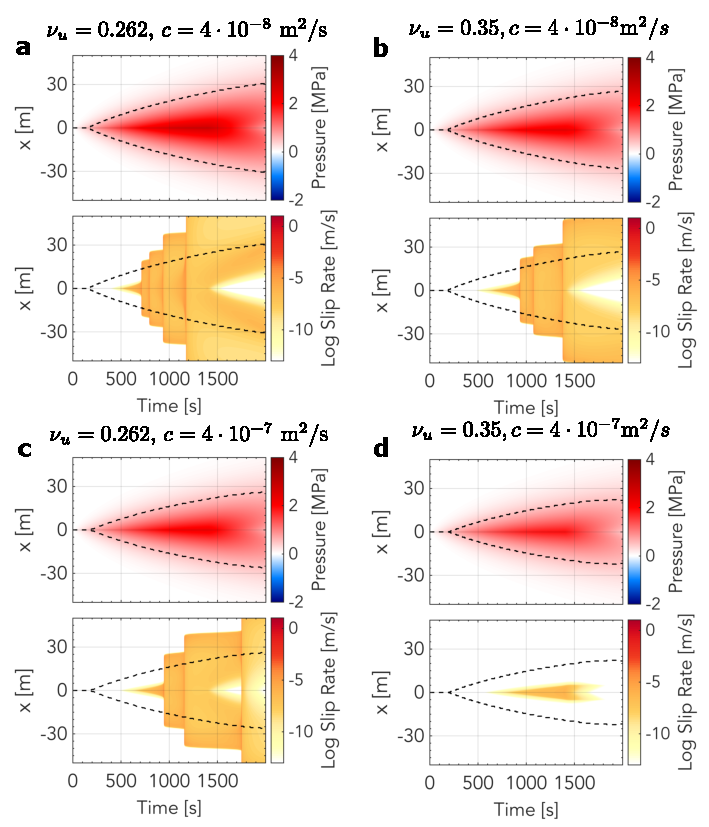
\includegraphics[scale = 0.95]{Figures/gamma0_comparison.pdf} % this command will be ignored
\caption{Simulations of fault fields with time and no dilatancy $\gamma = 0$ but varied bulk diffusivity $c$ and undrained Poisson's ratio $\nu_u$ as is listed above each panel. Each panel shows the average shear zone pressure $\langle p \rangle$ and log slip rate  $\log_{10}{V}$. $x$ indicates location along the length of the fault, but we note that the simulation domain is 5 times larger (400 m) than is shown. The black dashed lines are the 0.5 MPa pressure contours, which we take as representative of the pressure front distance. We observe highly stabilized slip in panel {\bf a}, where the undrained Poisson's ratio and the bulk diffusivity are larger. However, highly unstable slip in panel {\bf d} with {\bf a} smaller undrained Poisson's ratio and bulk diffusivity (four seismic events).}
\label{fig:Appg0}
\end{figure}

The simulations without dilatancy (Figure \ref{fig:Appg0}) demonstrate a wide spectrum of slip stability based on two parameters that have not been explored much in the literature: bulk diffusivity and undrained Poisson's ratio. First, with larger bulk diffusivity $c$ and undrained Poisson's ratio $\nu_u$ (panel {\bf a}) we observe very limited slip in response to the injection. Clearly, the fault is not slipping in a seismically unstable manner. In contrast, a smaller undrained Poisson's ratio $\nu_u$ and bulk diffusivity $c$ (panel d) result in highly unstable behavior with four seismic ruptures. In the two other cases, where one value is larger and the other smaller (panels {\bf b} and {\bf c}), we see similarly unstable behavior with three ruptures. This may indicate a degree of trade-off between  $\nu_u$ and $c$, and neither parameter alone is controlling the stability characteristics of the fault. This makes sense since $c$ will control the slip speed at which the bulk will respond in an undrained manner. We discuss how the undrained parameters play a significant role in the stability in section \ref{sec:undr}.

\subsection{Simulations with dilatancy $\gamma = 1.7 \cdot 10^{-5}$}

Here we explore the same parameter combinations, initial conditions, imposed injection, and overall setup as in Figure \ref{fig:Appg0}. However, we now include dilatancy setting $\gamma = 1.7 \cdot 10^{-5}$. This is 10\% of the standard value of $\gamma = 1.7 \cdot 10^{-4}$, which \citeA{Segall1995} derived from the experiments of \citeA{Marone1990}. $\gamma = 1.7 \cdot 10^{-4}$ is typically used in the literature and results using that value will be shown in the next section. However, we decided to explore a smaller value as it reveals an intermediate regime where slow slip outpaces the diffusion front (Figure \ref{fig:Appgs} )

\begin{figure}[H]
\centering
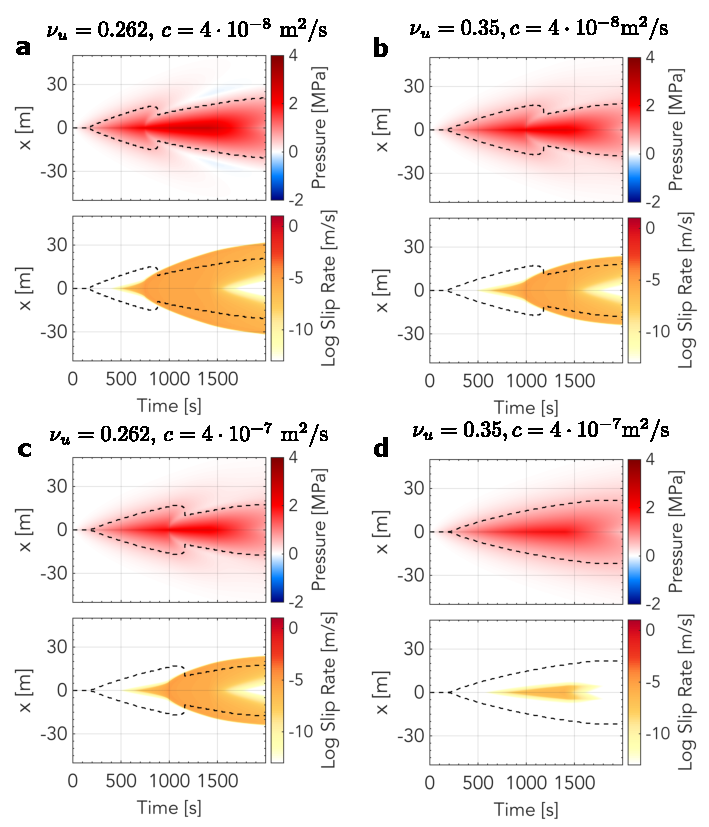
\includegraphics[scale =  0.95]{Figures/gammasmall_comparison.pdf} % this command will be ignored
\caption{
Simulations of fault fields with time and dilatancy $\gamma = 1.7 \cdot 10^{-5}$. Otherwise, the figures and simulation setup are the same as in Figure \ref{fig:Appg0}. We observe highly stabilized slip in panel a, where the undrained Poisson's ratio and the bulk diffusivity are larger. Here the results are largely consistent with those of Figure \ref{fig:Appg0} where panel {\bf a} shows very stable behavior, panel {\bf d} is the most unstable, and parameter combinations in panels {\bf b} and {\bf c} show similar stability. However, here all simulations show gradual migration of a slow slip front and no seismic event. Thus all simulations are substantially stabilized, as is expected from introducing dilatancy. We note negative pore pressure change at the slip-front in panel {\bf d}, and strong overall deviation from the square root characteristic growth of the pore pressure front. }
\label{fig:Appgs}
\end{figure}

It is notable in Figure \ref{fig:Appgs} that we observe similar effect of stabilization by changing $c$ and $\nu_u$ compared to Figure \ref{fig:Appg0}, with larger $\nu_u$ and $c$ showing high degree of stabilization (panel {\bf a}), but smaller $\nu_u$ and $c$ a developing instability, but panels {\bf b} and {\bf c} have similar levels of stability. However, in Figure \ref{fig:Appgs} the style of slip is very different. We observe no seismic events but slow slip migration. In all cases, except panel a, the slow slip outpaces the pore pressure front as indicated by the dashed 0.5 MPa contour. At the same time, the slip is drastically altering the pore pressure front. The influence of dilatancy on the fault pore pressure is most prominent in panel d, where the average pressure at the rupture tip is decreased compared to a background value, i.e. negative pore pressure change. The result is not a classic square-root-of-time diffusional pressure characteristic as is seen in Figure \ref{fig:Appg0} and Figure \ref{fig:Appgs}a but rather square-root characteristic initially, but once the slip speed is significant and the dilatancy alters the pore pressure and the characteristic is perturbed. The resulting shape of the fault pore pressure contour resembles the outline of a squid's head.  


\subsection{Simulations with dilatancy $\gamma = 1.7 \cdot 10^{-4}$}

Finally, we carry out simulations using the value of the dilatancy coefficient $\gamma = 1.7 \cdot 10^{-4}$ as inferred by \citeA{Segall1995}. This may be considered as a standard value as it is typically used. However, there is no general reason to believe that the dilatancy coefficient could not vary significantly. 

\begin{figure}[H]
\centering
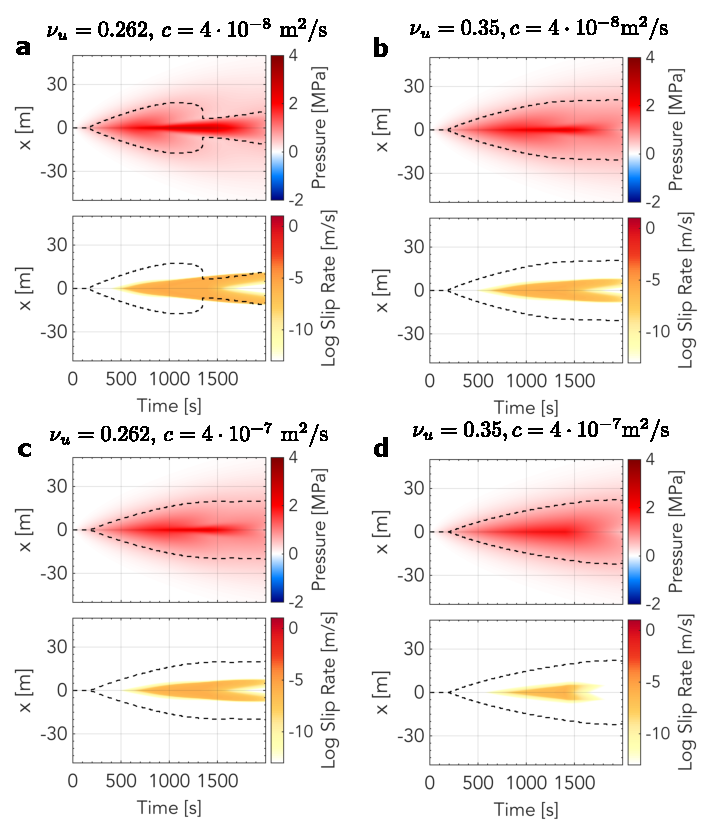
\includegraphics[scale =  0.95]{Figures/gammanorm_comparison.pdf} % this command will be ignored
\caption{Simulations of fault fields with time and dilatancy $\gamma = 1.7 \cdot 10^{-4}$. Otherwise the figures and simulation setup is the same as in Figure \ref{fig:Appg0}. We observe highly stabilized slip in all cases. Unlike the previous two cases the rupture only grows in a region of significantly elevated pore pressure. }
\label{fig:Appgn}
\end{figure}

For $\gamma = 1.7 \cdot 10^{-4}$ we observe highly stabilized slip (Figure \ref{fig:Appgn}). There is no seismic rupture and no slow slip front that is growing faster than the pore pressure diffuses. In other words, the rupture is driven in the location of high pore pressure and thus grows quasi-statically with the pressure front. Dilatancy influences the fault pressure, in particular in Figure \ref{fig:Appgn}d, but compared to Figure \ref{fig:Appgs} we observe that the dilatancy induced changes in pore pressure are less prominent in Figure \ref{fig:Appgn}. This may be somewhat counterintuitive given that the dilatancy coefficient is an order of magnitude larger in Figure \ref{fig:Appgn}. Since the dilatancy coefficient is smaller in Figure \ref{fig:Appgs} a larger slip patch can develop before dilatancy becomes significant. This slip patch is less stiff or alternatively one might state that it produces a higher energy release rate. Thus it is able to drive rupture propagation at a higher rate and more slip speed, which ultimately results in increased pore pressure response than when the dilatancy coefficient is larger and suppresses instability development at an earlier time. We emphasize that selecting $\gamma = 1.7 \cdot 10^{-4}$ does not generally mean stable rupture due to injection. Even if all the same parameters are selected, a seismic rupture could develop by simply altering the injection strategy; for example, injecting for a significantly longer time and at a higher rate would likely eventually lead to a seismic event.






\section{Discussion}

\subsection{Result summary and interpretation} \label{sec:undr}

The application of our method has had two main themes. First, by exploring how dilatancy affects the fault response due to injection. Second, how altering the bulk diffusivity and undrained Poisson's ratio influences the fault response from injection. Dilatancy is already understood to be a stabilizing mechanism \cite{Rudnicki1988,Segall1995,Segall2010b}, although limited study of coupled injection and dilatancy has been carried out \cite<except>{Ciardo2019,Yang2021}. Thus our general finding, that fault slip is stabilized and aseismic slip is promoted when dilatancy is included is not surprising. We have thus chosen to contrast this well-known stabilizing mechanism with less explored parameters that we are uniquely positioned to investigate with the method described in this paper. Namely we vary parameters $c$ and $\nu_u$. Indeed the latter has meaning only for a poroelastic solid. A purely elastic solid, as considered in most studies\cite<with some exceptions, e.g.>{Jha2014,Torberntsson2018,Heimisson2019} has only a single Poisson's ratio.

Our selection of three different $\gamma$ values reveals different modes of rupture. First, highly unstable response with repeated seismic ruptures of the same part of the fault. Second, slow slip migration that propagates beyond the pressurized region. Finally, quasi-statically growing slip only in regions of high pressure. This can be observed in Figures \ref{fig:Appg0}, \ref{fig:Appgs}, and \ref{fig:Appgn} respectively. The \citeA{Guglielmi2015} experiment reported primarily aseismic slip and significant dilatant behavior. Some micro-earthquakes were reported, but they may have been off the main fault and represent only a small fraction of the moment released. Thus our findings show, given the experimental constraints and information from a previous modeling study \cite{Larochelle2021} that inclusion of dilatancy results in behavior qualitatively similar to what was reported by \citeA{Guglielmi2015}. However, further study is needed for quantitative matching. We highlight that the method presented predicts fault opening from dilatancy or pressurization and thus may provide additional constraints in data application when that is directly measured \cite{Cappa2019}.

Our reported influence of bulk diffusivity and undrained Poisson's ratio is more novel. We observe that changing the bulk diffusivity by order of magnitude significantly stabilizes the fault in the simulations. It is important to emphasize that this result is also contingent on the shear zone mobility, which we have not systematically varied. This is due to the time scales of fluid diffusion in the bulk and shear zone are not independent as discussed by \citeA{Heimisson2021}. The bulk diffusivity has an important control on the stability of the fault as it will control how rapidly fluids can escape the shear zone. Our parameter choice (Appendix A) is such that it reflects a fault initially far from steady-state or, in other words, not critically stressed. Although the changes in average pressure in Figures  \ref{fig:Appg0}, \ref{fig:Appgs}, and \ref{fig:Appgn} are subtle, they are sufficient to cause significant stabilization in fault behavior. This can be observed by comparing panels {\bf a} and {\bf b}, or {\bf c} and {\bf d} in Figures \ref{fig:Appg0}, \ref{fig:Appgs}, and \ref{fig:Appgn}. 

Bulk diffusivity is often considered to be the same as that of the shear zone or the bulk is simply taken to be impermeable. In this study, we have taken what we consider to be small values of $c$, yet we observe a very significant effect. Further, as seen in equation (\ref{eq:pc}) the flux into the bulk scales with $\kappa_{cy}/\epsilon^2$. Since we expect $\epsilon$ the shear zone half-thickness to be small, we can expect that flux into the bulk occurs rapidly. Indeed in this study, we set the $\kappa_{cx}$, along shear zone mobility, to be a factor $10^9$ larger than $\kappa_{cy}$ such that the fluid migration along the shear zone was significant compared to the flux into the bulk. This highlights that how rapidly the bulk can transport fluids is critical for the fault dynamics. As discussed in \citeA{Heimisson2021}, and can be seen in the SBI solutions in this paper, the characteristic time of bulk diffusion is $\sim 1/(c k^2)$. Thus the bulk fluid transport is highly dependent on length scale, and idealizations of an impermeable bulk may only be valid at a certain length scale.

The dependence on the undrained Poisson's ratio may be surprising, and it may not be clear why having a pronounced undrained poroelastic response will result in a greater stabilization. The analysis of \citeA{Heimisson2021} provides some insight. The undrained critical wavenumber is 

\begin{equation}
|k_{cr}^{un}| \simeq \frac{2 \sigma_0(b-a)(1-\nu_u)}{GL} \left(1 - \frac{f_0 \gamma}{ \beta \sigma_0 (b-a) } + \mathcal{O}(\epsilon) \right) ,
\label{eq:kappa0un} 
\end{equation}

and the corresponding drained wavenumber is 

\begin{equation}
|k_{cr}^d| \simeq \frac{2 \sigma_0(b-a)(1-\nu)}{GL} \left(1 - \frac{f_0 \gamma}{ \beta \sigma_0 (b-a) } + \mathcal{O}(\epsilon) \right) ,
\label{eq:kappa0d} 
\end{equation}
assuming the shear zone mobility tends to zero. Thus the ratio of the minimum unstable wavelength in drained and undrained limits is

\begin{equation}
\frac{\lambda_d}{\lambda_{un}} = \frac{1 - \nu}{1 - \nu_u},
\end{equation}
Thus, at most, this ratio can be 2, but more commonly around 1 -- 1.5. In simple terms, it means that a perturbation or a slip patch on the fault of length $\Delta L$ may be unstable if the bulk responds in a drained manner. However, the patch or perturbation may need to be up to $2 \Delta L$ to be unstable if the bulk responds in an undrained manner. There are a few things to note about this stabilization. First, that it depends on the bulk diffusivity, length scale, and slip rate. The transition from a drained to undrained response will depend on the characteristic bulk diffusion time $\sim 1/(c k^2)$ relative to how fast the fault is slipping and the slip patch length scale (due to the $k^2$ dependence). Thus the timing of stabilization by a transition from drained to undrained response is nontrivial. Second, the drained and undrained limits are inadequate to characterize the stabilization fully. \citeA{Heimisson2021} showed that in an intermediate (neither drained nor undrained) regime, the fault could be more stable than in the undrained regime. Finally, since anti-plane sliding does not depend on Poisson's ratio, the same kind of stabilization will not occur. This may lead to interesting directional effects in 3D simulations. 

Panels {\bf b} and {\bf c} in Figures  \ref{fig:Appg0}, \ref{fig:Appgs}, and \ref{fig:Appgn} consistently show similar  rupture propagation and stabilization. This suggests that, in a certain sense, that setting $\nu_u = 0.35$ is approximately equally stabilizing as setting $c = 4 \cdot 10^{-7}$ m$^2$/s relative to the respective lower values in the simulation setup. Due to the many complexities mentioned in the previous paragraph we don't think this will hold generally. However, simulations with combined $\nu_u = 0.35$ and $c = 4 \cdot 10^{-7}$ m$^2$/s are nearly identical regardless of the $\gamma$ value ({\bf a} in Figures  \ref{fig:Appg0}, \ref{fig:Appgs}, and \ref{fig:Appgn} ). This observation highlights that bulk effects through combined diffusion and poroelasticity can be so stabilizing that dilatancy never becomes significant enough to affect the rupture propagation and nucleation.


\section{Conclusions}

We have presented novel spectral boundary-integral (SBI) solutions applicable to frictional and fracture mechanics problems in a plane strain linear poroelastic solid. The solutions consider that the interface of two poroelastic half-spaces may undergo mode I and II displacement discontinuity as well as pressurization. We have applied the solutions to develop a method and code implementation of a rate-and-state fault that has simultaneous inelastic dilatancy and injection. We apply this code to data from a field experiment, which has been previously analyzed by modeling. We explore the role of inelastic dilatancy, bulk diffusion, and poroelastic properties of the bulk on the simulation results. We find, surprisingly, that bulk diffusion and poroelastic properties of the bulk, which are parameters that are rarely explored, can qualitatively affect rupture stability and propagation. Further, we find the stabilization of bulk diffusion and poroelastic properties can be comparable to the well-known stabilizing dilatancy mechanism.


\section*{Data Availability Statement}
\noindent
 No original data is presented in this study. The data used in regard to application to the \cite{Guglielmi2015} field experiment was archived by \citeA{StacyData}: CaltechDATA repository (\url{https://data.caltech.edu/records/1891}). The software implementation of the method described in this paper is available here  \\ \noindent \url{https://doi.org/10.5281/zenodo.6010353} 
 \cite<see>{elias_rafn_heimisson_Poro_SBIM}.

\acknowledgments
This study was supported by the Geophysics Option Postdoctoral Fellowship from the Division of Geological and Planetary Sciences at Caltech and ETH Postdoctoral fellowship (Project No. FEL-19 20-2) to E.R.H. The work was further supported by the NSF-IUCRC Center for Geomechanics and Mitigation of Geohazards (projects GMG-4.1, GMG-4.2) to N.L.

\appendix
\section{Parameter values}
Here we briefly explain how the parameter values, listed in the table below, are set.

Parameters $G$, $\nu$, and all friction and loading parameters in Table \ref{symbolstable} are from \citeA{Larochelle2021}.
Compressibilities $\beta_f^p,\beta_f^\sigma,\beta_n^p,\beta_n^\sigma,\beta_g^p,\beta_g^\sigma$ in addition to $\phi_0$ and $\epsilon$ are selected as in \citeA{Heimisson2021}.

Skempton's coefficient is fixed and set to $0.85$, this value is representative of Westerly granite as well as certain types of sandstone and other rocks. The undrained Poisson's ratio is, on one hand, set to $0.35$ to reflect the approximate value of Westerly granite and on the other hand to 0.262 to represent the undrained value of Charcoal granite. We note that Charcoal granite has $\nu = 0.270$ and $\nu_u = 0.292$ \cite{Cheng2016}. However, we wish to fix $\nu$ such that we do have multiple parameters varying each simulation. Thus only the range $\nu_u - \nu$ is the same as for Charcoal granite albeit the Poisson's ratios are similar in absolute terms. Further, Charcoal granite has a substantially lower Skempton's coefficient $B = 0.454$, but we still use $B = 0.85$ again to limit the number of varying parameters. We, therefore, do not recommend using this paper as a reference for poroelastic parameters, but rather look at the overview of \citeA{Detournay1993,Cheng2016}, which we used, and references therein for more information on error and methods for measuring. Here we simply want to explore two cases where $\nu_u - \nu$ small and large, but at the same time make sure that the ranges reflect real values measured in rocks.

As explained in the main text, the range of the dilatancy coefficient is selected to reflect three different styles of ruptures. First we set $\gamma = 0$ and $\gamma = 1.7 \cdot 10^{-4}$ as trial values where the latter is the standard value used and was identified by \citeA{Segall1995}. We observed that the two values would typically render either highly unstable or very stable slip. Thus an value of $\gamma = 1.7 \cdot 10^{-5}$ was identified as producing sustained slow slip migration.

The two mobilities $\kappa_{cx}, \kappa_{cy}$ and the bulk hydraulic diffusivity $c$ were determined by trial and error by trying to approximately match the pore pressure evolution in \citeA{Larochelle2021}. We highlight that due to the heterogeneous permeability structure, the fact that we treat the pore pressure as non-constant in the shear zone, and other coupling mechanisms that alter the pore pressure, we cannot simply select parameters that give exactly the same pore pressure evolution as in \citeA{Larochelle2021}.


\begin{table}
\caption{Parameter values in the study}
\centering
%\resizebox{\textwidth}{!}{
\begin{tabular}{l l l}
\hline
Symbol & Description & Value\\
\hline
\multicolumn{3}{l}{\textit{Bulk and gouge material properties}}\\
$G$ & Shear modulus & 10 GPa\\
$B$ & Skempton's coefficient & 0.85\\
$\nu$ & Drained Poisson's ratio & 0.24\\
$\nu_u$ & Undrained Poisson's ratio & 0.35, 0.262\\
$\beta_f^p$,$\beta_f^\sigma$ & Isotropic and uniaxial fluid compressibility & $0.44 \cdot 10^{-9}$ Pa$^{-1}$, $0.24 \cdot 10^{-9}$ Pa$^{-1}$, \\
$\beta_n^p$,$\beta_n^\sigma$ & Isotropic and uniaxial pore volume compressibility & $6.0 \cdot 10^{-9}$ Pa$^{-1}$, $3.3 \cdot 10^{-9}$ Pa$^{-1}$, \\
$\beta_g^p$,$\beta_g^\sigma$ & Isotropic and uniaxial solid gouge compressibility & $0.020 \cdot 10^{-9}$ Pa$^{-1}$, $0.011 \cdot 10^{-9}$ Pa$^{-1}$, \\
$\phi_0$ & Reference porosity & 0.068 \\
$\gamma$ & Diltancy coefficient \cite{Segall1995} & 0, 1.7$\cdot$10$^{-5}$, 1.7$\cdot$10$^{-4}$ \\
$\epsilon$ & Shear-zone half thickness & 1.0 mm\\
$c$ & Bulk hydraulic diffusivity & 4$\cdot$10$^{-8}$, 4$\cdot$10$^{-7}$ m$^2$/s\\
$\kappa_{cx}$ & Along shear-zone mobility & 8.7584$\cdot$10$^{-11}$ m$^2$/(Pa s)\\
$\kappa_{cy}$ & Across shear-zone mobility & 8.7584$\cdot$10$^{-20}$ m$^2$/(Pa s)\\
\multicolumn{3}{l}{\textit{Friction and loading parameters}}\\
$L$ & Characteristic state evolution distance & 16.75 $\mu$m \\
$a$ & Direct rate dependence of friction & 0.01125\\
$b$ & State dependence of friction &  0.016 \\
$\alpha_{LD}$ & \citeA{Linker1992} constant &  0.0 \\
$V_0$ & reference slip rate & $10^{-6}$~m/s \\
$f_0$ & reference friction & 0.55 \\
$\tau_0$ & Initial shear stress & 2.15 MPa \\
$\sigma_0$ & Initial effective normal stress & 4 MPa \\
\hline
\end{tabular}
\label{symbolstable}
\end{table}

\section{Method validation}

The spectral boundary-integral method, in addition to the rate-and-state fault slip simulations, couples together several physical processes that could not be simulated with another individual code. Further, no analytical solutions are available that also couple all these processes. It is, therefore, nearly impossible to benchmark and test all capabilities of the code and implementation simultaneously. However, here we list to provide an overview of the tests and validation we carried out.

\begin{itemize}
    \item As was reported in Figure \ref{fig:Song} the SBI solutions for $\tau'$ and $p^\pm$ were tested against the solutions of \cite{Song2017}.
    \item The analytical inversion of the Laplace transform was in all cases tested by also numerically inverting the Laplace transform numerically using the Talbot method \cite{Talbot1979}
    \item Using $p^+$ as the relevant pore pressure when computing the effective normal stress, we reproduced the results of \cite{Heimisson2019}, which were done with a different code \cite{Torberntsson2018}. We, for example, reproduced the spontaneously occurring instabilities at mildly rate-strengthening friction that give rise to slow-slip pulses, which only occur in a limited parameter regime. Our results were consistent with the spatial dimension of the instabilities and the pulse propagation speeds as reported by \cite{Heimisson2019}.
    \item Using the linearized stability analysis of \cite{Heimisson2021} we identified the critical wavenumber for many different regimes, such as high diffusivity, low diffusivity, intermediate diffusivity as well as thicker and thinner shear zones. In the code, a fully non-linear implementation, we induced a critical wavelength perturbation, as determined by the linearized analysis, by introducing a small perturbation in the initial state around steady-state sliding. We found in all cases that the perturbation in the slip speed oscillated without growing or decaying.
\end{itemize}

The tests and benchmarking above do validate most aspects of the implementation and method we have introduced in this paper. However, none test the injection into the fault and fluid propagation as a result of the injection. In order to check the robustness of the algorithm in this regard, we set up a problem with injection and delayed nucleation with dilatancy. The simulations are run until the slip speed reaches 1 cm/s, which we take as the instability time. This setup thus tests how well the pore pressure injection and subsequent diffusion is resolved as it promotes instability. We generate a manufactured solution with the error tolerance and state integration parameter set to $\xi = 1/4096$ (see section \ref{sec:time}). Then setting $\xi \in \{ 1/4, 1/8, 1/16, 1/32, 1/64  \}$ and investigating the $L_1$ norm error of the manufactured solution and the less accurate solutions plotted against the total number of iterations (which scales with the computational time) we see a second-order convergence. Where we look at the time of instability, the slip speed profile at the instability time, the $p_c$ value at the instability time, and the slip profile at that time. $\xi = 1/32$ roughly correspond to a relative error of $10^{-3}$ in all the fields we looked at, but we stress that the magnitude of the relative error depends on the problem and the simulation time. For simulations we favor using $\xi = 1/32$ and one minimum iteration (see section \ref{sec:time} for discussion on iterations). If smaller values than $\xi = 1/64$ are compared to the manufactured solution, the convergence gets more complicated but tends to improve to the first order with the iteration number. Using no minimum iteration or 2 minimum iterations also works and gives consistent results. We suggest 1 minimum iteration is most efficient in terms of obtaining a stable convergent solution at the fewest total iterations.

Finally, we note that Figure \ref{fig:Appg0}c demonstrates, by chance, that the simulations are well resolved and accurate. A careful inspection of the figures shows that the last event is not one event but two events nucleating at exactly the same time around $x \approx \pm 30$ m and then coalescing. While such a high degree of symmetry is not physically realistic, it is a strong indication of well-resolved simulations in time and space, especially when it occurs not at the first simulated event. The same phenomenon also occurs in Figure \ref{fig:Appg0}b, but it is not as clear.


\newpage

\bibliography{agusample}




\end{document}



More Information and Advice:

%% ------------------------------------------------------------------------ %%
%
%  SECTION HEADS
%
%% ------------------------------------------------------------------------ %%

% Capitalize the first letter of each word (except for
% prepositions, conjunctions, and articles that are
% three or fewer letters).

% AGU follows standard outline style; therefore, there cannot be a section 1 without
% a section 2, or a section 2.3.1 without a section 2.3.2.
% Please make sure your section numbers are balanced.
% ---------------
% Level 1 head
%
% Use the \section{} command to identify level 1 heads;
% type the appropriate head wording between the curly
% brackets, as shown below.
%
%An example:
%\section{Level 1 Head: Introduction}
%
% ---------------
% Level 2 head
%
% Use the \subsection{} command to identify level 2 heads.
%An example:
%\subsection{Level 2 Head}
%
% ---------------
% Level 3 head
%
% Use the \subsubsection{} command to identify level 3 heads
%An example:
%\subsubsection{Level 3 Head}
%
%---------------
% Level 4 head
%
% Use the \subsubsubsection{} command to identify level 3 heads
% An example:
%\subsubsubsection{Level 4 Head} An example.
%
%% ------------------------------------------------------------------------ %%
%
%  IN-TEXT LISTS
%
%% ------------------------------------------------------------------------ %%
%
% Do not use bulleted lists; enumerated lists are okay.
% \begin{enumerate}
% \item
% \item
% \item
% \end{enumerate}
%
%% ------------------------------------------------------------------------ %%
%
%  EQUATIONS
%
%% ------------------------------------------------------------------------ %%

% Single-line equations are centered.
% Equation arrays will appear left-aligned.

Math coded inside display math mode \[ ...\]
 will not be numbered, e.g.,:
 \[ x^2=y^2 + z^2\]

 Math coded inside \begin{equation} and \end{equation} will
 be automatically numbered, e.g.,:
 \begin{equation}
 x^2=y^2 + z^2
 \end{equation}


% To create multiline equations, use the
% \begin{eqnarray} and \end{eqnarray} environment
% as demonstrated below.
\begin{eqnarray}
  x_{1} & = & (x - x_{0}) \cos \Theta \nonumber \\
        && + (y - y_{0}) \sin \Theta  \nonumber \\
  y_{1} & = & -(x - x_{0}) \sin \Theta \nonumber \\
        && + (y - y_{0}) \cos \Theta.
\end{eqnarray}

%If you don't want an equation number, use the star form:
%\begin{eqnarray*}...\end{eqnarray*}

% Break each line at a sign of operation
% (+, -, etc.) if possible, with the sign of operation
% on the new line.

% Indent second and subsequent lines to align with
% the first character following the equal sign on the
% first line.

% Use an \hspace{} command to insert horizontal space
% into your equation if necessary. Place an appropriate
% unit of measure between the curly braces, e.g.
% \hspace{1in}; you may have to experiment to achieve
% the correct amount of space.


%% ------------------------------------------------------------------------ %%
%
%  EQUATION NUMBERING: COUNTER
%
%% ------------------------------------------------------------------------ %%

% You may change equation numbering by resetting
% the equation counter or by explicitly numbering
% an equation.

% To explicitly number an equation, type \eqnum{}
% (with the desired number between the brackets)
% after the \begin{equation} or \begin{eqnarray}
% command.  The \eqnum{} command will affect only
% the equation it appears with; LaTeX will number
% any equations appearing later in the manuscript
% according to the equation counter.
%

% If you have a multiline equation that needs only
% one equation number, use a \nonumber command in
% front of the double backslashes (\\) as shown in
% the multiline equation above.

% If you are using line numbers, remember to surround
% equations with \begin{linenomath*}...\end{linenomath*}

%  To add line numbers to lines in equations:
%  \begin{linenomath*}
%  \begin{equation}
%  \end{equation}
%  \end{linenomath*}



%Here we demonstrate and application of the methodology to better understand earthquake triggering and nucleation into a fault in response to injection with and without dilatancy.

%\subsection{Problem Setup}

%The problem setup is similar to what is shown in the schematic Figure \ref{fig:schema}a. Fluid mass is injected into a region of from  $x = -5$ m to $x = 5$ m  at the origin of the x-axis. The frictional fault is 300 m long, with imposed creeping regions slipping at $V = V_0 = 10^{-9}$ m/s of 100 m on either side of the frictional domain. The fault is initially at steady-state sliding, no initial perturbation is added to the system other than the injection. In this exercise we vary only one parameter, the mass injection rate $\dot{Q}$, with the additional constraint that we only inject a fixed mass of water of 0.36 kg per unit length in the invariant direction ($z$-axis). During the injection the rate is constant and then abruptly turned off when the fixed amount of mass is reached. We explore a large range in injection duration ranging from 1 minute to 1 month, thus ranging 4 orders of magnitude in injection rate. We simulate the nucleation of the first event and stop all simulations after the first seismic even when slip speed has started decreasing.


%Parameters are as indicated in Table \ref{symbolstable}. It's worth highlighting that here we have assumed chosen the shear-zone mobility to be strongly anisotropic with $\kappa_{cx}$ 9 orders of magnitude larger than $\kappa_{cy}$. This is, firstly, motivated by idea that highly sheared fault zones may act as  barriers for fluid flow across them but conduits for flow along the fault zone. Secondly, we wanted to demonstrate that the method could provide a stable solution for such a large mobility difference.

%\subsection{Results}

%We first explore the slip-speed evolution following an injection in two case: 1 minute injection (Figure \ref{fig:time}ab) and 1 week injection (Figure \ref{fig:time}cd). First, we observe remarkably small difference between not included dilatancy and including dilatancy Figure \ref{fig:time} a,c vs. b,d). This simply means that most of the time from injection to nucleation, the dilatancy effect is negligible. However, as will be apparent in Figure \ref{fig:simcomb}, that if the same results are plotted with the time-step number on the $y$-axis significant then differences are revealed since the dilatancy reponse will only affect the rupture when the slip speed is approaching seismic levels.

%\begin{figure}[H]
%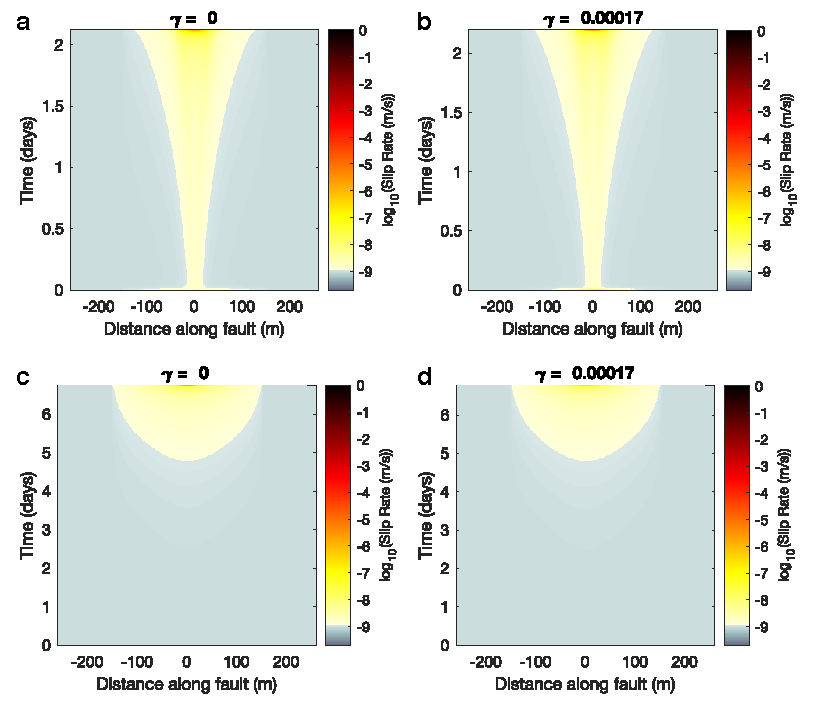
\includegraphics[scale = 1]{Figures/time_comparison.pdf} % this command will be ignored
%\caption{Slip rate, shown as color in a $\log_{10}$ scale, on fault with time for 1 minute injection duration (top row, a, b) and 1 week injection duration (bottom row, c, d). Further, we show the response without dilatancy (a,c) and with dilatancy. We note, that as plotted it appears that dilatancy has not effect on slip speed evolution, but this is not true, as is disscuss in this section. One can observe signification deferences in slip-speed evolution depending on the injection duration. For rapid injection (a,b) the nucleation of a seismic even happens around day 2 for slow injection (c,d) closer to 1 week time. }
%\label{fig:time}
%\end{figure}

%Viewing the simulation results in terms of simulation time-step number, but not physical time, is useful to reveal processes that may happen quickly compared to the nucleation time. Figure \ref{fig:simcomb} shows slip speed (a,d), cumulative slip (b,e), and average shear zone pore pressure (c,f), for injection and conditions (1 minute injection) except one case doesn't include dilatancy (a,b,c) and the other includes dilatancy (d,e,f). Comparing to Figure \ref{fig:time}, where the results look nearly identical, we now observe substantial differences. First in the slip speed we observe a more gradual expansion of the nucleation region in the simulation with dilatancy (d), this is suggesting greater accumulation of aseismic slip. Indeed the slip during the earthquake is less for the diltancy case compared to the non-dilatancy case (e vs. b). This difference will be further analyzed in Figure \ref{fig:allcomb}. Further, the average pore pressure evolves differently as expected. The only change in average pore pressure for the no dilatancy, $\gamma = 0$, occurs in the beginning due to the injection (c). That pore pressure then quickly diffuses into the bulk. Exactly the same change occurs in the dilatancy, $\gamma = 1.7\cdot10^{-4}$, this change appears to be shorter but that is only because the y-axis is different as is discussed in the next paragraph. The average pore pressure change in the two cases deviates only when the slip speed has reached about $\sim 10^{-5}$ m/s. At this point the diffusion along the shear zone and along the bulk doesn't equilibrate the pore pressure decrease sufficiently fast such that the pressure in the shear zone drops, it is only at this point that the two cases become significantly difference.

%We highlight that the simulation with dilatancy requires more time-step, but here the $y$-axis represent every 50th true time-step taken in the simulation. Thus a simulation, in this case, with dilatancy requiers about 4 time as many time steps. This is because, as nucleation is ongoing the pore pressure continuously changes, and the algorithm needs refinement for accuracy. However, most of the time-steps the pore pressure doesn't change significantly because the dilatancy induced pore pressure changes are equilibrated by the bulk (Figure \ref{fig:simcomb}e).

%\begin{figure}[H]
%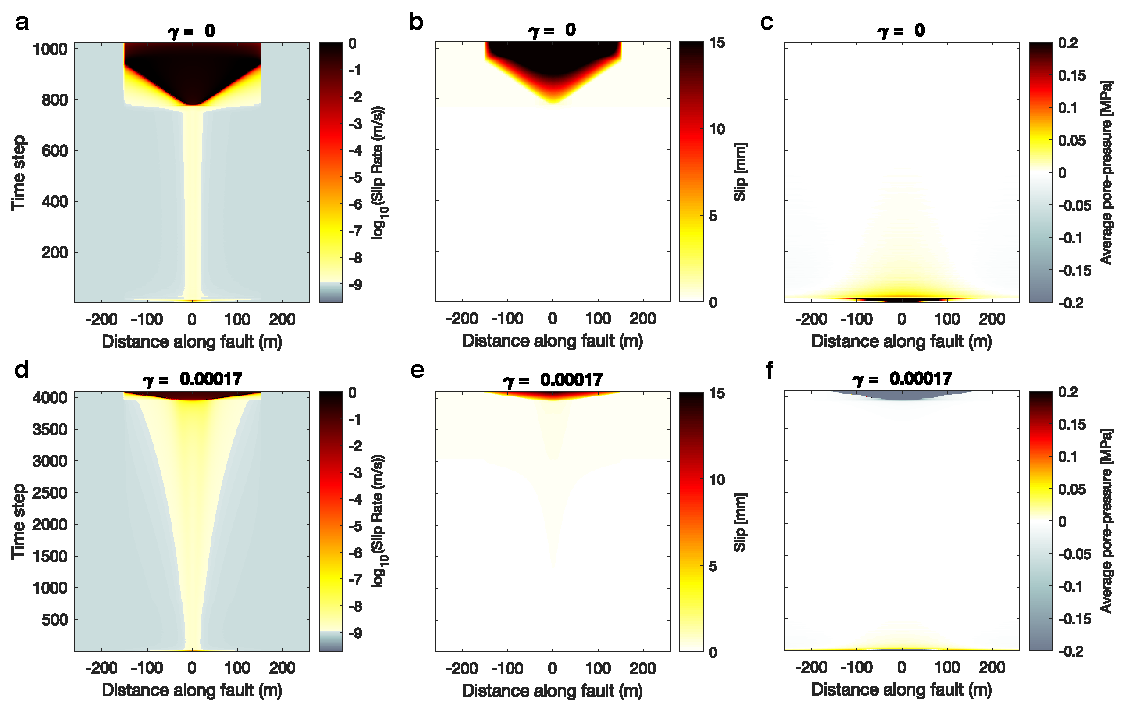
\includegraphics[scale = 0.8]{Figures/simulation_compare.pdf} % this command will be ignored
%\caption{Comparison of different fault fields as a function of time-step, for identical simulation (1 minute injection time) with and without dilatancy. Log-slip speed $\log_{10} (V)$ (a,d), cumulative slip $\delta$ (b,e), and average shear zone pore pressure $\langle p \rangle$ (c,f). Diltancy is omitted by setting $\gamma = 0$ (a,b,c), but included with $\gamma = 1.7\cdot10^{-4}$ (d,e,f). Note that color scales doe not represent the full range for better visualization. Solid black or dark grey incorporate values beyond the range of the color scales.}
%\label{fig:simcomb}
%\end{figure}

%Two prominent and current questions in the study of induced earthquakes are: 1) does injection strategy the timing and size of an induced earthquake. 2) What is the role of dilatancy in injection induced seismicity? Here we explore these questions by running simulations (such as show in Figures \ref{fig:time} and \ref{fig:simcomb}) for injection durations ranging from 1 minute to 1 month. As was previously mentioned, the duration in changed but not the mass injected. 

%The relationship between the injection duration and the timing of the earthquake is explored in Figure \ref{fig:allcomb}a. We observe that once the injection duration exceeds 1 day, there is a dependence of the two resembling a square-root function. However at a shorter injection duration there is an abrupt drop in the event time. The one-to-one line on the plot demonstrates that if the dots occur on the right-hand side of the lone it means that the seismic event occurs during the injection. However, if the dots occur on the left-hand side they occur after injection stops. This leads to a conclusion that might be perceived as counter intuitive, which is that if you inject the mass rapidly the seismic event happens after you stop injecting. For example, if the mass is all injected in 1 minute, the event still takes about 50 hours to become and earthquake. This delay is simply the manifestation of other time-dependent processes as the unstable slip patch takes time to grow and reach a critical dimension. Such a possible delay between injection and nucleation is often not accounted for in simplified models of induced seismicity. A striking feature is the overlap of the blue and orange dots indicating that dilatancy isn't affecting the time the event occurs. This is simply relecting what was observed in Figure \ref{fig:time} and \ref{fig:simcomb}) that dilatancy, in this problem, isn't important until at later stages in the nucleation process when slip speed is relatively large. However, Figure \ref{fig:allcomb}a demonstrates that this is true for all the tested injection duration. 

%Figure \ref{fig:allcomb}b explores the average slip that occurs while the fault is slipping at seismic slip speeds (here taken as 1 cm/s or higher).

%\begin{figure}[H]
%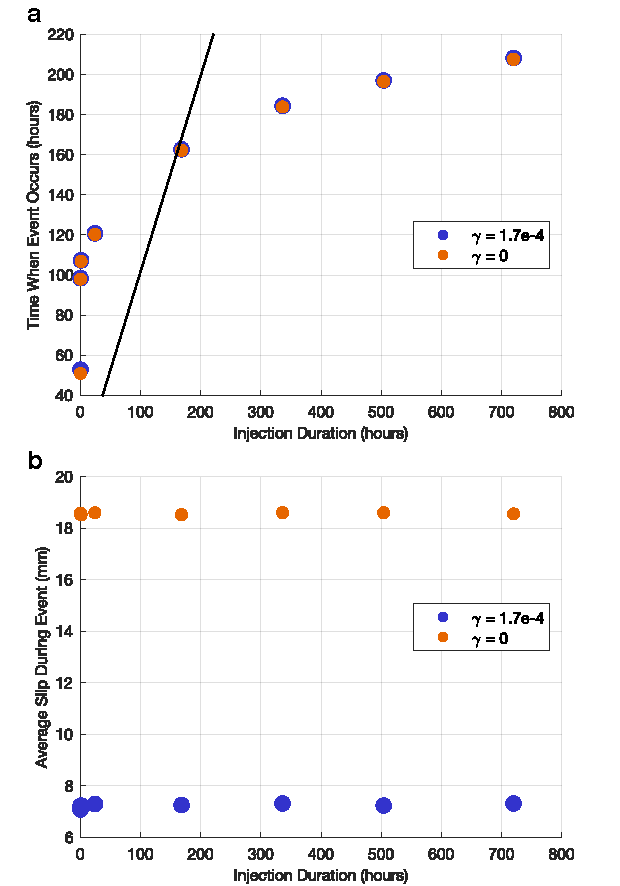
\includegraphics[scale = 1]{Figures/Instability_overview.pdf} % this command will be ignored
%\caption{}
%\label{fig:allcomb}
%\end{figure}